%  A simple AAU report template.
%  2015-05-08 v. 1.2.0
%  Copyright 2010-2015 by Jesper Kjær Nielsen <jkn@es.aau.dk>
%
%  This is free software: you can redistribute it and/or modify
%  it under the terms of the GNU General Public License as published by
%  the Free Software Foundation, either version 3 of the License, or
%  (at your option) any later version.
%
%  This is distributed in the hope that it will be useful,
%  but WITHOUT ANY WARRANTY; without even the implied warranty of
%  MERCHANTABILITY or FITNESS FOR A PARTICULAR PURPOSE.  See the
%  GNU General Public License for more details.
%
%  You can find the GNU General Public License at <http://www.gnu.org/licenses/>.
%
%  A simple AAU report template.
%  2015-05-08 v. 1.2.0
%  Copyright 2010-2015 by Jesper Kjær Nielsen <jkn@es.aau.dk>
%
%  This is free software: you can redistribute it and/or modify
%  it under the terms of the GNU General Public License as published by
%  the Free Software Foundation, either version 3 of the License, or
%  (at your option) any later version.
%
%  This is distributed in the hope that it will be useful,
%  but WITHOUT ANY WARRANTY; without even the implied warranty of
%  MERCHANTABILITY or FITNESS FOR A PARTICULAR PURPOSE.  See the
%  GNU General Public License for more details.
%
%  You can find the GNU General Public License at <http://www.gnu.org/licenses/>.
%
\documentclass[11pt,twoside,a4paper,openright]{report}
%%%%%%%%%%%%%%%%%%%%%%%%%%%%%%%%%%%%%%%%%%%%%%%%
% Language, Encoding and Fonts
% http://en.wikibooks.org/wiki/LaTeX/Internationalization
%%%%%%%%%%%%%%%%%%%%%%%%%%%%%%%%%%%%%%%%%%%%%%%%
% Select encoding of your inputs. Depends on
% your operating system and its default input
% encoding. Typically, you should use
%   Linux  : utf8 (most modern Linux distributions)
%            latin1 
%   Windows: ansinew
%            latin1 (works in most cases)
%   Mac    : applemac
% Notice that you can manually change the input
% encoding of your files by selecting "save as"
% an select the desired input encoding. 
\usepackage[utf8]{inputenc}
% Make latex understand and use the typographic
% rules of the language used in the document.
\usepackage[danish,english]{babel}
% Use the palatino font
\usepackage[sc]{mathpazo}
\linespread{1.05}         % Palatino needs more leading (space between lines)
% Choose the font encoding
\usepackage[T1]{fontenc}
%%%%%%%%%%%%%%%%%%%%%%%%%%%%%%%%%%%%%%%%%%%%%%%%
% Graphics and Tables
% http://en.wikibooks.org/wiki/LaTeX/Importing_Graphics
% http://en.wikibooks.org/wiki/LaTeX/Tables
% http://en.wikibooks.org/wiki/LaTeX/Colors
%%%%%%%%%%%%%%%%%%%%%%%%%%%%%%%%%%%%%%%%%%%%%%%%
% load a colour package
\usepackage{xcolor}
\definecolor{aaublue}{RGB}{33,26,82}% dark blue
% The standard graphics inclusion package
\usepackage{graphicx}
% Set up how figure and table captions are displayed
\usepackage{caption}
\captionsetup{%
  font=footnotesize,% set font size to footnotesize
  labelfont=bf % bold label (e.g., Figure 3.2) font
}
% To use subfigures
\usepackage{subcaption}
% Make the standard latex tables look so much better
\usepackage{array,booktabs}
\usepackage{float}
% Enable the use of frames around, e.g., theorems
% The framed package is used in the example environment
\usepackage{framed}

%%%%%%%%%%%%%%%%%%%%%%%%%%%%%%%%%%%%%%%%%%%%%%%%
% Mathematics
% http://en.wikibooks.org/wiki/LaTeX/Mathematics
%%%%%%%%%%%%%%%%%%%%%%%%%%%%%%%%%%%%%%%%%%%%%%%%
% Defines new environments such as equation,
% align and split 
\usepackage{amsmath}
% Adds new math symbols
\usepackage{amssymb}
% double brackets [[, \\llbracket \\rrbracket
\usepackage{stmaryrd}
% Use theorems in your document
% The ntheorem package is also used for the example environment
% When using thmmarks, amsmath must be an option as well. Otherwise \eqref doesn't work anymore.
\usepackage[framed,amsmath,thmmarks]{ntheorem}
%algoritms
\usepackage{algorithmicx,algpseudocode}
\algdef{SE}[DOWHILE]{Do}{doWhile}{\algorithmicdo}[1]{\algorithmicwhile\ #1}%

% listings used for code examples
\usepackage{listings}
% default style
\lstdefinestyle{default}{
  numbers=left,
  frame=single,
  captionpos=b,
}
% python style
\lstdefinestyle{python}{
  style=default,
  language=Python,
  basicstyle=\small\tt,
  keywordstyle=\color{blue},
  commentstyle=\color[rgb]{0.13,0.54,0.13},
  backgroundcolor=\color{cyan!10},
  morekeywords={
    True,
    False
    },
}
%%%%%%%%%%%%%%%%%%%%%%%%%%%%%%%%%%%%%%%%%%%%%%%%
% Page Layout
% http://en.wikibooks.org/wiki/LaTeX/Page_Layout
%%%%%%%%%%%%%%%%%%%%%%%%%%%%%%%%%%%%%%%%%%%%%%%%
% Change margins, papersize, etc of the document
\usepackage[
  inner=28mm,% left margin on an odd page
  outer=41mm,% right margin on an odd page
  ]{geometry}
% Modify how \chapter, \section, etc. look
% The titlesec package is very configureable
\usepackage{titlesec}
\titleformat{\chapter}[display]{\normalfont\huge\bfseries}{\chaptertitlename\ \thechapter}{20pt}{\Huge}
\titleformat*{\section}{\normalfont\Large\bfseries}
\titleformat*{\subsection}{\normalfont\large\bfseries}
\titleformat*{\subsubsection}{\normalfont\normalsize\bfseries}
%\titleformat*{\paragraph}{\normalfont\normalsize\bfseries}
%\titleformat*{\subparagraph}{\normalfont\normalsize\bfseries}

% Clear empty pages between chapters
\let\origdoublepage\cleardoublepage
\newcommand{\clearemptydoublepage}{%
  \clearpage
  {\pagestyle{empty}\origdoublepage}%
}
\let\cleardoublepage\clearemptydoublepage

% Change the headers and footers
\usepackage{fancyhdr}
\pagestyle{fancy}
\fancyhf{} %delete everything
\renewcommand{\headrulewidth}{0pt} %remove the horizontal line in the header
\fancyhead[RE]{\small\nouppercase\leftmark} %even page - chapter title
\fancyhead[LO]{\small\nouppercase\rightmark} %uneven page - section title
\fancyhead[LE,RO]{\thepage} %page number on all pages
% Do not stretch the content of a page. Instead,
% insert white space at the bottom of the page
\raggedbottom
% Enable arithmetics with length. Useful when
% typesetting the layout.
\usepackage{calc}

\usepackage[natbib=true, style=numeric, backend=bibtex, sorting=none,maxbibnames=99]{biblatex}
\addbibresource{bib/mybib}


%%%%%%%%%%%%%%%%%%%%%%%%%%%%%%%%%%%%%%%%%%%%%%%%
% Misc
%%%%%%%%%%%%%%%%%%%%%%%%%%%%%%%%%%%%%%%%%%%%%%%%
% Add bibliography and index to the table of
% contents
\usepackage[nottoc]{tocbibind}
% Add the command \pageref{LastPage} which refers to the
% page number of the last page
\usepackage{lastpage}
% Add todo notes in the margin of the document
\usepackage[
%  disable, %turn off todonotes
  colorinlistoftodos, %enable a coloured square in the list of todos
  textwidth=\marginparwidth, %set the width of the todonotes
  textsize=scriptsize, %size of the text in the todonotes
  ]{todonotes}

%%%%%%%%%%%%%%%%%%%%%%%%%%%%%%%%%%%%%%%%%%%%%%%%
% Hyperlinks
% http://en.wikibooks.org/wiki/LaTeX/Hyperlinks
%%%%%%%%%%%%%%%%%%%%%%%%%%%%%%%%%%%%%%%%%%%%%%%%
% Enable hyperlinks and insert info into the pdf
% file. Hypperref should be loaded as one of the 
% last packages
\usepackage{hyperref}
\hypersetup{%
	pdfpagelabels=true,%
	plainpages=false,%
	pdfauthor={Author(s)},%
	pdftitle={Title},%
	pdfsubject={Subject},%
	bookmarksnumbered=true,%
	colorlinks=false,%
	citecolor=black,%
	filecolor=black,%
	linkcolor=black,% you should probably change this to black before printing
	urlcolor=black,%
	pdfstartview=FitH%
}

% Custom commands
% Project tool/program name
\newcommand{\pyt}{\text{PyT}}

\newcommand{\ppv}[4]{\begin{figure}[h]
   \centering
\begin{tikzpicture}
  \node[circle] (var) at (0,5) {#1};
  \node[draw, line width=0.05mm, minimum width=1cm,minimum height=1cm, outer sep=10pt] (mem) at (1.5,5) {mem};
  \node (result) at (3,5) {#2};
  \draw[->] (var) -- (mem);
  \draw[->] (result) -- (mem);
\end{tikzpicture}   
  \caption{#3}
  \label{#4}
\end{figure}
}


% Should always be loaded last
\usepackage{cleveref}
\crefname{listing}{listing}{listings}
\crefname{figure}{figure}{figures}
% package inclusion and set up of the document
% see, e.g., http://en.wikibooks.org/wiki/LaTeX/Formatting#Hyphenation
% for more information on word hyphenation
\hyphenation{ex-am-ple hy-phen-a-tion short}
\hyphenation{long la-tex}
% 
%  A simple AAU report template.
%  2015-05-08 v. 1.2.0
%  Copyright 2010-2015 by Jesper Kjær Nielsen <jkn@es.aau.dk>
%
%  This is free software: you can redistribute it and/or modify
%  it under the terms of the GNU General Public License as published by
%  the Free Software Foundation, either version 3 of the License, or
%  (at your option) any later version.
%
%  This is distributed in the hope that it will be useful,
%  but WITHOUT ANY WARRANTY; without even the implied warranty of
%  MERCHANTABILITY or FITNESS FOR A PARTICULAR PURPOSE.  See the
%  GNU General Public License for more details.
%
%  You can find the GNU General Public License at <http://www.gnu.org/licenses/>.
%
%
%
% see, e.g., http://en.wikibooks.org/wiki/LaTeX/Customizing_LaTeX#New_commands
% for more information on how to create macros

%%%%%%%%%%%%%%%%%%%%%%%%%%%%%%%%%%%%%%%%%%%%%%%%
% Macros for the titlepage
%%%%%%%%%%%%%%%%%%%%%%%%%%%%%%%%%%%%%%%%%%%%%%%%
%Creates the aau titlepage
\newcommand{\aautitlepage}[3]{%
  {
    %set up various length
    \ifx\titlepageleftcolumnwidth\undefined
      \newlength{\titlepageleftcolumnwidth}
      \newlength{\titlepagerightcolumnwidth}
    \fi
    \setlength{\titlepageleftcolumnwidth}{0.5\textwidth-\tabcolsep}
    \setlength{\titlepagerightcolumnwidth}{\textwidth-2\tabcolsep-\titlepageleftcolumnwidth}
    %create title page
    \thispagestyle{empty}
    \noindent%
    \begin{tabular}{@{}ll@{}}
      \parbox{\titlepageleftcolumnwidth}{
        \iflanguage{danish}{%
          
\includegraphics[width=\titlepageleftcolumnwidth]{figures/aau_logo_da}
        }{%
          
\includegraphics[width=.9\titlepageleftcolumnwidth]{figures/aau_logo_en}
        }
      } &
      \parbox{\titlepagerightcolumnwidth}{\raggedleft\sf\small
        #2
      }\bigskip\\
       #1 &
      \parbox[t]{\titlepagerightcolumnwidth}{%
      \textbf{Abstract:}\bigskip\par
        \fbox{\parbox{\titlepagerightcolumnwidth-2\fboxsep-2\fboxrule}{%
          #3
        }}
      }\\
    \end{tabular}

    \noindent \textbf{Source code:}\\ \url{https://github.com/SW10IoT/pyt/tree/finalfinal}    
    \vfill
    \iflanguage{danish}{%
      \noindent{\footnotesize\emph{Rapportens indhold er frit tilgængeligt, men offentliggørelse (med kildeangivelse) må kun ske efter aftale med forfatterne.}}
    }{%
      \noindent{\footnotesize\emph{The content of this report is freely available, but publication (with reference) may only be pursued due to agreement with the author.}}
    }
    \clearpage
  }
}

%Create english project info
\newcommand{\englishprojectinfo}[8]{%
  \parbox[t]{\titlepageleftcolumnwidth}{
    \textbf{Title:}\\ #1\bigskip\par
    \textbf{Theme:}\\ #2\bigskip\par
    \textbf{Project Period:}\\ #3\bigskip\par
    \textbf{Project Group:}\\ #4\bigskip\par
    \textbf{Participant(s):}\\ #5\bigskip\par
    \textbf{Supervisor(s):}\\ #6\bigskip\par
    \textbf{Page Numbers:} \pageref{LastPage}\bigskip\par
    \textbf{Date of Completion:}\\ #8
  }
}

%Create danish project info
\newcommand{\danishprojectinfo}[8]{%
  \parbox[t]{\titlepageleftcolumnwidth}{
    \textbf{Titel:}\\ #1\bigskip\par
    \textbf{Tema:}\\ #2\bigskip\par
    \textbf{Projektperiode:}\\ #3\bigskip\par
    \textbf{Projektgruppe:}\\ #4\bigskip\par
    \textbf{Deltager(e):}\\ #5\bigskip\par
    \textbf{Vejleder(e):}\\ #6\bigskip\par
    \textbf{Oplagstal:} #7\bigskip\par
    \textbf{Sidetal:} \pageref{LastPage}\bigskip\par
    \textbf{Afleveringsdato:}\\ #8
  }
}

%%%%%%%%%%%%%%%%%%%%%%%%%%%%%%%%%%%%%%%%%%%%%%%%
% An example environment
%%%%%%%%%%%%%%%%%%%%%%%%%%%%%%%%%%%%%%%%%%%%%%%%
\theoremheaderfont{\normalfont\bfseries}
\theorembodyfont{\normalfont}
\theoremstyle{break}
\def\theoremframecommand{{\color{gray!50}\vrule width 5pt \hspace{5pt}}}
\newshadedtheorem{exa}{Example}[chapter]
\newenvironment{example}[1]{%
		\begin{exa}[#1]
}{%
		\end{exa}
}

\newcommand{\constraint}[1]{
\llbracket #1 \rrbracket
  }

\newcommand{\assignconstraint}[3]{
#1 ~ \downarrow ~ #2 ~ \cup ~ #3
  }
% my new macros
\theoremheaderfont{\normalfont\bfseries}
\theorembodyfont{\normalfont}
\theoremstyle{break}
\def\theoremframecommand{{\color{gray!50}\vrule width 5pt \hspace{5pt}}}

\newshadedtheorem{defini}{Definition}[chapter]
\newenvironment{definition}[1]{%
    \begin{defini}[#1]
}{%
    \end{defini}
}


\begin{document}
%frontmatter
\pagestyle{empty} %disable headers and footers
\pagenumbering{roman} %use roman page numbering in the frontmatter
%  A simple AAU report template.
%  2015-05-08 v. 1.2.0
%  Copyright 2010-2015 by Jesper Kjær Nielsen <jkn@es.aau.dk>
%
%  This is free software: you can redistribute it and/or modify
%  it under the terms of the GNU General Public License as published by
%  the Free Software Foundation, either version 3 of the License, or
%  (at your option) any later version.
%
%  This is distributed in the hope that it will be useful,
%  but WITHOUT ANY WARRANTY; without even the implied warranty of
%  MERCHANTABILITY or FITNESS FOR A PARTICULAR PURPOSE.  See the
%  GNU General Public License for more details.
%
%  You can find the GNU General Public License at <http://www.gnu.org/licenses/>.
%
\pdfbookmark[0]{Front page}{label:frontpage}%
\begin{titlepage}
  \addtolength{\hoffset}{0.5\evensidemargin-0.5\oddsidemargin} %set equal margins on the frontpage - remove this line if you want default margins
  \noindent%
  \begin{tabular}{@{}p{\textwidth}@{}}
    \toprule[2pt]
    \midrule
    \vspace{0.2cm}
    \begin{center}
    \Huge{\textbf{
        PyT
    }}
    \end{center}
    \begin{center}
      \Large{A Static Analysis Tool for Detecting Security Vulnerabilities in Python Web Applications
      }
    \end{center}
    \vspace{0.2cm}\\
    \midrule
    \toprule[2pt]
  \end{tabular}
  \vspace{4 cm}
  \begin{center}
    {\large
      Master's Thesis%Insert document type (e.g., Project Report)
    }\\
    \vspace{0.2cm}
    {\Large
    Stefan Micheelsen, Bruno Thalmann%Insert your group name or real names here
    }
  \end{center}
  \vfill
  \begin{center}
  Aalborg University\\
  Computer Science
  \end{center}
\end{titlepage}
\clearpage

\thispagestyle{empty}
{\small
\strut\vfill % push the content to the bottom of the page
\noindent Copyright \copyright{} Aalborg University 2015\par
\vspace{0.2cm}
\noindent Here you can write something about which tools and software you have used for typesetting the document, running simulations and creating figures. If you do not know what to write, either leave this page blank or have a look at the colophon in some of your books.
}
\clearpage


\pdfbookmark[0]{English title page}{label:titlepage_en}
\aautitlepage{%
  \englishprojectinfo{
    Project Title %title
  }{%
    Scientific Theme %theme
  }{%
    Spring Semester 2016 %project period
  }{%
    des106f16 % project group
  }{%
    %list of group members
    Stefan Micheelsen\\ 
    Bruno Thalmann
  }{%
    %list of supervisors
    René Rydhof Hansen\\
    Mads Chr. Olesen
  }{%
    1 % number of printed copies
  }{%
    \today % date of completion
  }%
}{%department and address
  \textbf{Computer Science}\\
  Aalborg University\\
  \href{http://www.aau.dk}{http://www.aau.dk}
}{% the abstract
  Here is the abstract
}

\cleardoublepage
\pdfbookmark[0]{Contents}{label:contents}
\pagestyle{fancy} %enable headers and footers again
\tableofcontents
\listoftodos
\chapter*{Preface\markboth{Preface}{Preface}}\label{ch:preface}
\addcontentsline{toc}{chapter}{Preface}
This master's thesis has been prepared by 10th semester Software Engineering students at Aalborg University, during the spring-semester of 2016.
It is expected of the reader to have a background in IT/software, due to the technical content.

References and citations are done by the use of numeric notation, e.g. [1], which refers to the first item in the bibliography.

We would like to thank our supervisor René Rydhof Hansen and co-supervisor Mads Chr. Olesen for their excellent supervision throughout the project period.
\vspace{\baselineskip}\hfill Aalborg University, \today

\cleardoublepage
%mainmatter
\pagenumbering{arabic} %use arabic page numbering in the mainmatter

\chapter{Introduction}\label{ch:introduction}
\chapter{Introduction}\label{ch:introduction}
Here is the introduction. The next chapter is chapter~\ref{ch:ch2label}.


a new paragraph


\section{Examples}
You can also have examples in your document such as in example~\ref{ex:simple_example}.
\begin{example}{An Example of an Example}
  \label{ex:simple_example}
  Here is an example with some math
  \begin{equation}
    0 = \exp(i\pi)+1\ .
  \end{equation}
  You can adjust the colour and the line width in the {\tt macros.tex} file.
\end{example}

\section{How Does Sections, Subsections, and Subsections Look?}
Well, like this
\subsection{This is a Subsection}
and this
\subsubsection{This is a Subsubsection}
and this.

\paragraph{A Paragraph}
You can also use paragraph titles which look like this.

\subparagraph{A Subparagraph} Moreover, you can also use subparagraph titles which look like this\todo{Is it possible to add a subsubparagraph?}. They have a small indentation as opposed to the paragraph titles.

\todo[inline,color=green]{I think that a summary of this exciting chapter should be added.}
 % intro

\chapter{Preliminaries}
In order to analyze a Flask application it is necessary to have a basic understanding of both the Flask framework and the Python programming language.
In addition we need to have an understanding of the security vulnerabilities that we want to detect.

This chapter will attempt to make an introductory course in Python and flask, first covering the basics and then describing the important constructs that will be used in the report.
Afterwards it will describe the vulnerabilities that our tool is supposed to detect.

\section{Existing Tools}
In this section we attempt to look at tools that find security vulnerabilities by analysing Python web applications.
We have found two tools which are described in the following.

\subsection{Python Taint Mode}
The Python Taint Mode, \citet{conti2010taint}, is a 300 LOC library which contains a series of functions that are used as decorators to taint the source code.
To use the library one has to decorate the source code.
Also for variables a function \texttt{taint} is used to taint them.
Using this tool means one has to go through the whole source code and taint, variables and functions.
The tool can not handle booleans and has some built in class function it can not handle.
The effectiveness of the tool is not documented.

\subsection{Rough Auditing Tool for Security}
The Rough Auditing Tool for Security(RATS)

\section{Python Web Frameworks}
This section contains some of the available Python web frameworks.
The web frameworks are chosen from \citet{python_web_frameworks_list}.

\section{Why Flask}
This section argues why the the Flask web framework was chosen.
Flask is a small framework where the developer has a lot of power on how to structure and do things.
The framework is easy to grasp although it can be tough to master.
A factor to take into account is that the project group has previous experience using Flask.
This is an important factor as the project is about finding security vulnerabilities so the choice of framework is not that significant.
Another important factor is the simplicity of Flask.
This simplicity enables us to focus on the important task at hand and not how to develop a web app.


\chapter{Python}
\section{Python}\label{python}
This section will shortly give an overview of the Python programming language version 3.5.1.
This section is based on \citet{python_docs}.

\subsection{About Python}
The Python programming language is a dynamic, interpreted programming language created by Guido van Rossum in the early 1990s.
Python supports multiple programming paradigms, including object oriented and functional programming.
The design philosophy of python values code readability and expressivity.

\subsection{Parsing Python}
A Python program uses newlines as delimiters between statements.\footnote{A line can be joined with the next line if it has a ``\texttt{\textbackslash}'' at the end of the line.}
But if an expression is stretched over several lines for instance in parentheses it is still one line but several physical lines.
A comment starts with a ``\texttt{\#}'' symbol.
Indentation is used for grouping statements for instance a body of a function.
A file is a module which contains definitions and statements and ends with the suffix \texttt{.py}.
A program can contain several modules.

\subsection{Objects}
All data in Python is represented as objects.
An object consists of an identity, a type and a value.
The identity of an object never changes and is represented as an integer.
The type of an object defines how the object can be used and which operations are supported by the object.
The value of an object can for some objects change.
Objects whose value can be changed are called mutable, while objects whose value can not be changed are immutable.

Definition of objects happen in class definitions.
Classes have methods and attributes attached to it.
In \cref{class_definition} a class is defined.
The \texttt{\_\_init\_\_()} method is an initializer function which is called when a new instance is created of that class.
The \texttt{self} keyword references instance variables and instance methods.
This example defines the \texttt{MyClass} class which has one instance method \texttt{print\_i} and one instance variable \texttt{i}.
An instance of this class is created with the value five passed to the \texttt{i} variable through the initializer.
The \texttt{print\_i()} instance method is then called, which will print the value of \texttt{i}.

\begin{lstlisting}[style=python, caption={Class definition}, label=class_definition]
def MyClass(object):
    def __init__(self, i):
        self.i = i

    def print_i(self):
        print('Now i is:' +  i)

mc = MyClass(5)
mc.print_i()        
\end{lstlisting}

\subsection{Collections}
Python contains a number of built in collection classes used to store items in a structured way.
The following will shortly describe the most common collections and their uses, based on \citet{python_datastructures} where additional information can also be found.
The mentioned operations will be exemplified in \cref{collections}.


\paragraph{Lists} A list is a mutable sequence of items.
A list can be appended and extended items, and membership testing can be performed with the \texttt{in} keyword.
A list is iterable and can be indexed to retrieve individual items.
Lists are created with square brackets or the \texttt{list()} function.

\paragraph{Tuples} A tuple is similar to a list, but is an immutable sequence of a number of values.
A tuple is created with round brackets or the \texttt{tuple()} function.

\paragraph{Sets} A set is an implementation of the mathematical set.
It is an unordered collection that contains no duplicates.
A set is created with curly brackets or the \texttt{set()} function.

\paragraph{Dictionaries} A dictionary is an associative map, mapping a key to an item.
The key can be any immutable type which can then be extracted as when indexing a list.
Dictionaries are constructed with curly brackets contained key-value pairs or with the \texttt{dict()} function.

\begin{lstlisting}[style=python, caption={Usage of Python collections}, label=collections]
l = [1, 2, 3, 4] # a list of 4 elements - 1, 2, 3, 4
l.append(9) # append to the list -> 1, 2, 3, 4, 9

s = (5, 6, 7, 8, 8, 8, 8) # a set of 4 elements - 5, 6, 7, 8
l.extend(s) # extend the list with the set
            # -> 1, 2, 3, 4, 10, 5, 6, 7, 8

l.sort() # sort the list
l # the sorted list -> 1, 2, 3, 4, 5, 6, 7, 8, 9

t1 = (1,2) # a tuple -> (1,2)
t1[1] # retrieve the element at index 1 -> 2

t2 = (3,4) # another tuple -> (3,4)

d = dict([t1,t2]} # creating a dictionary from a list of tuples
                  # -> {1 : 2, 3 : 4}
d[1] # retrive item at key 1 - 2
  
d[1] in l # membership testing. Is 2 in l? -> True
    
for element in l: # iterating over the list
    print(element) 
    
\end{lstlisting}

\subsection{Control Structures}\label{python:control_structures}
The python programming language has three control structures, \texttt{if}, \texttt{while} and \texttt{for}.
In the following they are presented with simple code examples and a figure showing the possible information flow through the control structure.

\paragraph{If}
The \texttt{if} control structure has several variants:
\begin{enumerate}
\item A simple \texttt{if} statement
\item An \texttt{if-else} statement
\item An \texttt{if-elif-else} statement where the \texttt{elif} statement can be repeated
\end{enumerate}

\Cref{python:if:simple} shows a simple \texttt{if} control structure containing only one \texttt{if} statement.
The code, \cref{python:if:simple:code}, is an \texttt{if} statement with a condition, \texttt{True}.
If the condition holds the body is executed and if not, the program moves on to the next piece of code.
This flow is depicted on \cref{python:if:simple:flow}.

\begin{figure}[H]
  \centering
  \begin{subfigure}[b]{0.4\textwidth}
    \begin{lstlisting}[style=python]
if True:
    x = 0
    \end{lstlisting}
    \caption{Code example.}
    \label{python:if:simple:code}
  \end{subfigure}
  ~ %add desired spacing between images, e. g. ~, \quad, \qquad, \hfill etc. 
  %(or a blank line to force the subfigure onto a new line)
  \begin{subfigure}[b]{0.4\textwidth}
    \centering
    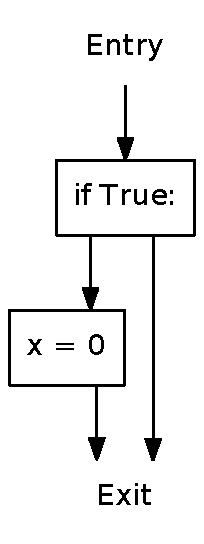
\includegraphics[scale=.4]{./figures/if.pdf}
    \caption{Possible flows.}
    \label{python:if:simple:flow}
  \end{subfigure}
  \caption{A simple \texttt{if} control structure containing one \texttt{if} statement.}
  \label{python:if:simple}
\end{figure}

The two other variants of the \texttt{if} control structure utilize the \texttt{else} clause to define what should be executed if the condition is \texttt{False}.
This \texttt{else} clause can be a statement body, or a nested \texttt{if} which is denoted as an \texttt{elif}.
An example of this can be seen on \cref{python:if:elif}.
The outmost \texttt{if} has a nested \texttt{elif} statement which then contains a body executed when the \texttt{elif} condition evaluates to \texttt{True} and an \texttt{else} executed when it evaluates to \texttt{False}.


\begin{figure}[H]
  \centering
  \begin{subfigure}[b]{0.4\textwidth}
    \begin{lstlisting}[style=python]
if True:
    x = 0
elif False:
    y = 0
else:
    z = 0
    \end{lstlisting}
    \caption{Code example.}
    \label{python:if:elif:code}
  \end{subfigure}
  ~ %add desired spacing between images, e. g. ~, \quad, \qquad, \hfill etc. 
  %(or a blank line to force the subfigure onto a new line)
  \begin{subfigure}[b]{0.4\textwidth}
    \centering
    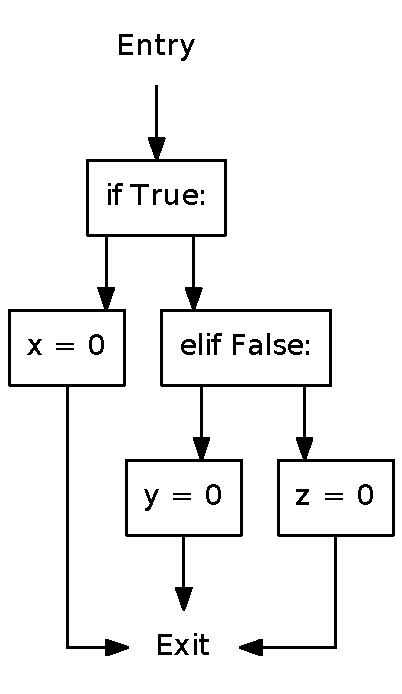
\includegraphics[scale=.4]{./figures/if_else_elif.pdf}
    \caption{Possible flows.}
    \label{python:if:elif:flow}
  \end{subfigure}
  \caption{An \texttt{if} control structure containing an \texttt{if}, an \texttt{elif}, and an \texttt{else} statement.}
  \label{python:if:elif}
\end{figure}



\paragraph{While}
The \texttt{while} control structure has a condition which evaluates to true or false.
If the condition is true the body is executed and the condition is evaluated again, if it still holds the body is executed again.
This process continuous until the condition is false.
A \texttt{while} control structure can also have an \texttt{else} clause.
The body of the \texttt{else} clause is executed when the condition of the \texttt{while} statement is false.

An example is displayed in \cref{python:while:else} which contains a  \texttt{while} control structure with the condition \texttt{x > 100} and an \texttt{else} clause.
The possible flows can be seen on \cref{python:while:else:flow}, where the \texttt{else} clause is executed when the condition resolves to \texttt{False}
\todo{vi mangler break logikken}

\begin{figure}[H]
  \centering
  \begin{subfigure}[b]{0.4\textwidth}
    \begin{lstlisting}[style=python, caption={Code example.}, label={python:while:else:code}]
while x < 100:
    x += 1
    x += 2
else:
    x += 3
    x += 4
    \end{lstlisting}
  \end{subfigure}
  ~ %add desired spacing between images, e. g. ~, \quad, \qquad, \hfill etc. 
  %(or a blank line to force the subfigure onto a new line)
  \begin{subfigure}[b]{0.4\textwidth}
    \centering
    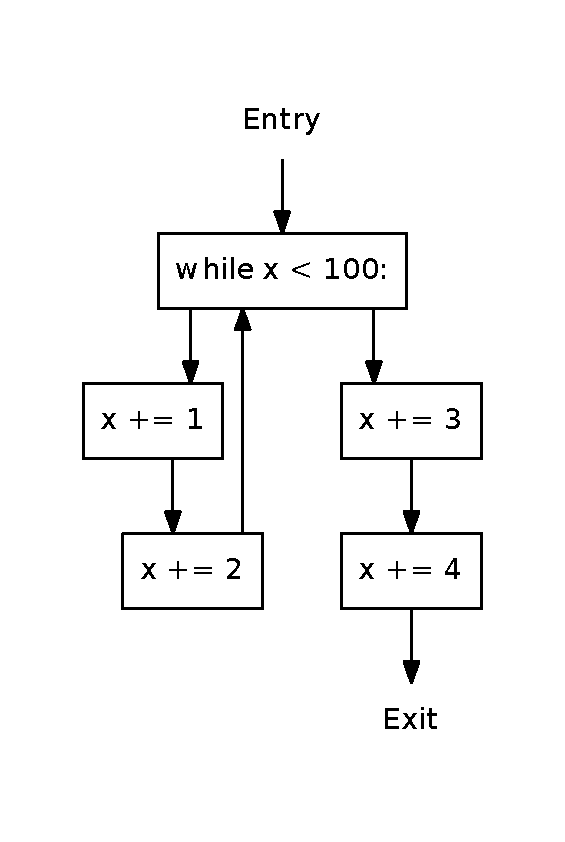
\includegraphics[scale=.4]{./figures/while_else.pdf}
    \caption{Possible flows.}
    \label{python:while:else:flow}
  \end{subfigure}
  \caption{A \texttt{while} control structure.}
  \label{python:while:else}
\end{figure}


\paragraph{For}
The \texttt{for} control structure is used for iterating over an object that is iterable.
This could for instance be a list or a tuple.
This control structure has an optional \texttt{else} statement, which body is executed when there is nothing to iterate or the \texttt{for} statement is done iterating.
To illustrate the \texttt{for} control structure we provide two examples.
The first example, on \cref{python:for}, shows the most common usage of the \texttt{for} control structure.
Here we iterate over a range, which is a built in function that returns a range of numbers, in this case 0, 1 and 2.
The second example also has a \texttt{else} statement and can be found on \cref{python:for:else}.
\todo{som de ser ud nu er de meget ens, og to virker overflodigt. Igen mangler vi break til at forklare else clause}

\begin{figure}
  \centering
  \begin{subfigure}[b]{0.4\textwidth}
    \begin{lstlisting}[style=python, caption={Code example.}, label={python:for:code}]
for x in range(3):
    print(x)
    y += 1
x = 3
    \end{lstlisting}
  \end{subfigure}
  ~ %add desired spacing between images, e. g. ~, \quad, \qquad, \hfill etc. 
  %(or a blank line to force the subfigure onto a new line)
  \begin{subfigure}[b]{0.4\textwidth}
    \centering
    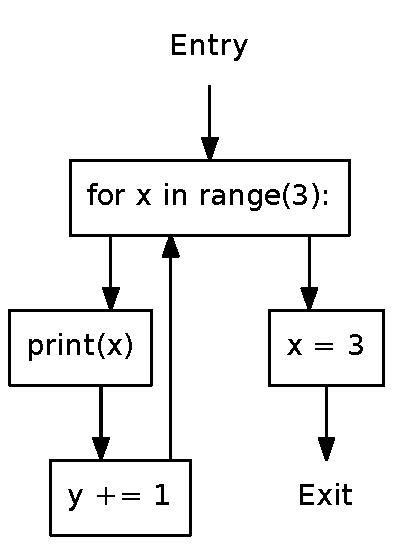
\includegraphics[scale=.5]{./figures/for.pdf}
    \caption{Possible flows.}
    \label{python:for:flow}
  \end{subfigure}
  \caption{A \texttt{for} control structure.}
  \label{python:for}
\end{figure}


\begin{figure}
  \centering
  \begin{subfigure}[b]{0.4\textwidth}
    \begin{lstlisting}[style=python, caption={Code example.}, label={python:for:else:code}]
for x in range(3):
    print(x)
    y += 1
else:
    print(y)
    \end{lstlisting}
  \end{subfigure}
  ~ %add desired spacing between images, e. g. ~, \quad, \qquad, \hfill etc. 
  %(or a blank line to force the subfigure onto a new line)
  \begin{subfigure}[b]{0.4\textwidth}
    \centering
    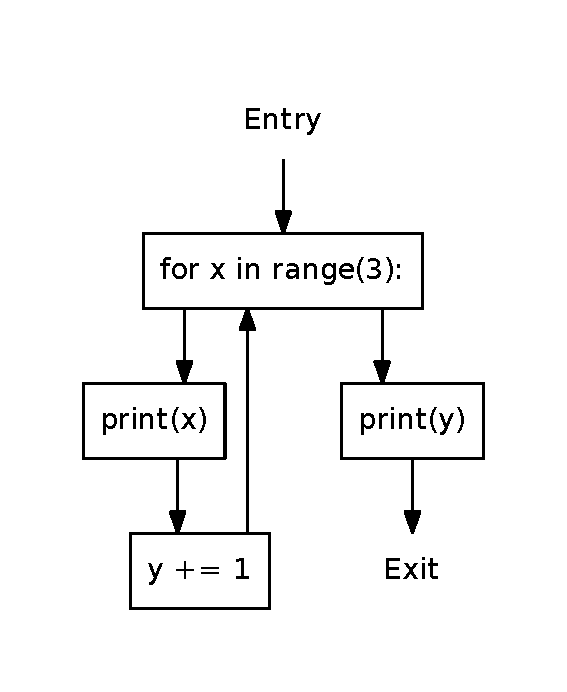
\includegraphics[scale=.5]{./figures/for_complete.pdf}
    \caption{Possible flows.}
    \label{python:for:else:flow}
  \end{subfigure}
  \caption{A \texttt{for} control structure with an \texttt{else} statement.}
  \label{python:for:else}
\end{figure}

\section{Surprising features in Python}
When working so close to the specification of a language some weird or surprising structures in the language arise.
While we programmed the conversion from abstract syntax tree to a control flow graph, we had these experiences once in a while, and working with the structures has given us some insight, both in the workings of python and in the details of these interesting structures.
This section will discuss some of these experiences.

\subsection{While - else}
Normally we know \texttt{while} as a simple control structure that has a condition and a body.
The body will execute until the condition is false.
This implementation is also found in Python, but Python has an extra variant of the while loop - an else clause.
An example of a while loop with an else clause can be seen on \cref{surprise_while_else}.

\begin{figure}
  \centering
  \begin{subfigure}[b]{0.4\textwidth}
    \begin{lstlisting}[style=python]
while x < threshold:
    if invalid_value(x):
        break
    x += 1
else:
    handle_value()
    \end{lstlisting}
    \caption{A while loop with an else clause}\label{surprise_while_else}
    \end{subfigure}
  ~
    \begin{subfigure}[b]{0.4\textwidth}
      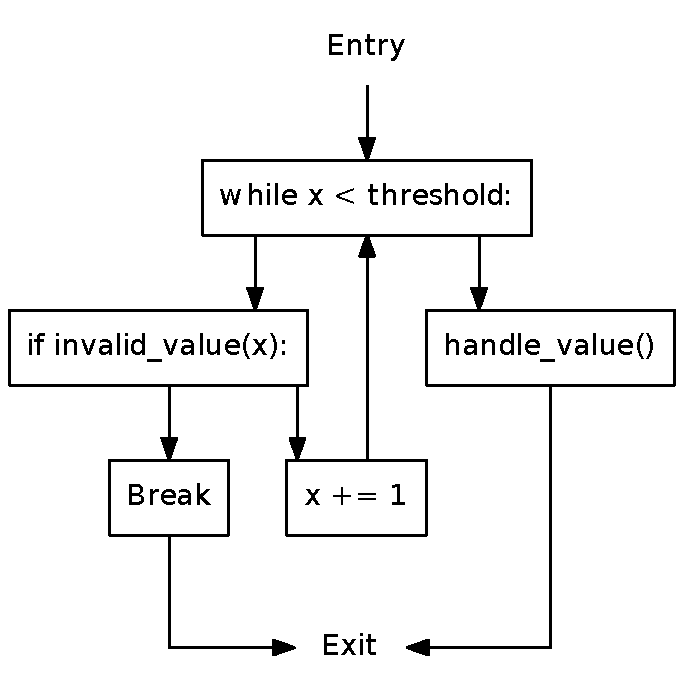
\includegraphics[scale=.5]{./figures/while_break.pdf}
      \caption{Possible flows}\label{surprise_while_else_cfg}
    \end{subfigure}
    
  \caption{An example of a while loop with a break statement}
\end{figure}


The else clause will execute when the condition is false, but if the body is exited by a \texttt{break} statement, the else clause will not be executed.
In the example in \cref{surprise_while_else}, this is being utilised to handle values that are unexpected in some way.
If that is the case, we break the body and do not execute the else clause which contains some logic for the value behaved as expected.

The \texttt{for} loop in Python also has an \texttt{else} clause which works in the same way.
A example of this can be seen in \cref{python:for:else}.

\begin{figure}
  \centering
  \begin{subfigure}[b]{0.4\textwidth}
    \begin{lstlisting}[style=python]
for x in range(5):
    if invalid_value(x):
        break
    print(x)
else:
    print('Accepted')
    \end{lstlisting}
    \caption{Code example}\label{python:for:else:code}
  \end{subfigure}
  ~ %add desired spacing between images, e. g. ~, \quad, \qquad, \hfill etc. 
  %(or a blank line to force the subfigure onto a new line)
  \begin{subfigure}[b]{0.4\textwidth}
    \centering
    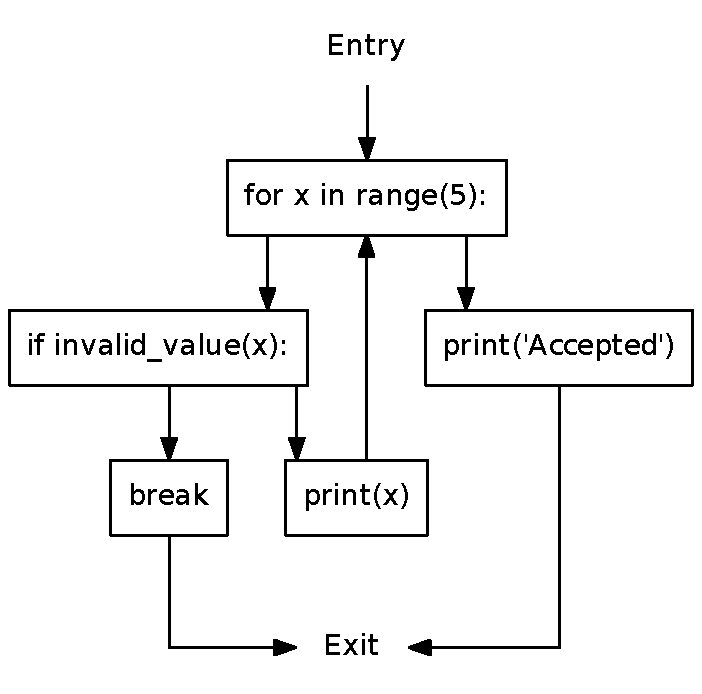
\includegraphics[scale=.5]{./figures/for_else.pdf}
    \caption{Possible flows}
    \label{python:for:else:flow}
  \end{subfigure}
  \caption{A \texttt{for} control structure with an \texttt{else} statement}
  \label{python:for:else}
\end{figure}

\subsection{Generator expression}
The Python language has a goal of being simple, explicit and readable\citep{python_zen}.
This can often be seen in some very elegant constructions contained in the language.
One of those is the generator statement, which was discovered during the development of \pyt{}.

A generator expression is a concise notation for a common pattern: iterating over a collection of items and then performing some operation on every element\citep{python_functional}.

\begin{lstlisting}[style=python, caption={Generator expression, stripping white-space from strings}, label={generator_strip}]
strings = ['King Arthur   ', '', '   Queen Elizabeth',
           '', '   Arnold Schwarzenegger   ']

people = (line.strip() for line in strings if line != '')
\end{lstlisting}

In \cref{generator_strip} some file has been parsed into an array.
The resulting strings have some undesirable white-space, and some of the strings are even empty.
The subsequent generator expression handles both of these problems.

A generator expression consists of an expression part and a for part.
The for part is evaluated and the expression is executed on each element of the resulting iterable.
The result is a generator that contains the results.

In \cref{generator_strip} the generator iterates over the strings with the \texttt{for} statement and filters out empty strings with the \texttt{if} statement.
The resulting elements are the stripped of white-space by the initial expression.

The generator in \cref{generator_strip} can be written without using a generator expression.
This can be seen in \cref{generator_corresponding}.
The generator expression is very clear in conveying its purpose while being shorter than the ``old way''.
\begin{lstlisting}[style=python, caption={\Cref{generator_strip} implemented without using an generator expression}, label={generator_corresponding}]
for line in strings:
    if not line != '':
        yield line.strip()
\end{lstlisting}

Python contains similar constructs called the comprehensions which return a list, set or dictionary of the element instead of a generator.
This construct uses square or curly parenthesis instead of round parenthesis, but are not different in any other way.
An example of a list comprehension can be seen in \cref{listcomp}.

\begin{lstlisting}[style=python, caption={The generator from \cref{generator_strip} changed to a list comprehension}, label={listcomp}]
people = [line.strip() for line in strings if line != '']
\end{lstlisting}

\subsection{Parameter Passing}
This section describes how Python deals with parameter passing.
This is included as we were surprised how it is dealt with and it is important to factor in when parameters are assigned in functions.

The most known parameter passing techniques are pass-by-reference and pass-by-value.
A short description of these to will lead up to an explanation of how Python is handling parameter passing.

\paragraph{Pass-by-reference}
\paragraph{Pass-by-value}
\paragraph{Pass-by-object-reference}



\chapter{Flask}
\section{Flask}
Flask is a framework for developing web applications in python\citep{flask_official}.
Its goal is to be minimal without compromising functionality.
It is extensible and flexible, so components like database, template engine and form validation can be chosen by the developer.

The minimal nature of Flask makes it possible to write a web page in a very small amount of code.
The following program, see \cref{minimal_flask}, creates a web server that serves a ``Hello World!'' page on the root.

\begin{lstlisting}[style=python, caption={Minimal Flask application}, label={minimal_flask}]
from flask import Flask
app = Flask(__name__)

@app.route('/')
def hello_world():
    return 'Hello World!'

if __name__ == '__main__':
    app.run()
\end{lstlisting}

The Flask framework is imported and a function is defined with the \texttt{app.route} decorator \todo{beskriv decorators i python intro} which tells the framework where to serve the page.
The function returns the string ``Hello World!'' which is shown on the web page.

The following will present the Flask functionality that will be used in this project.
The descriptions will be based on the \citet{flask_docs}.

\paragraph{Routing}
The \texttt{app.route} decorator is used to bind a function to a URL.
The parameter provided binds the function to the relative path.
Example paths are '/' for the root and '/hello\_world' for a sub-page.
The example in \cref{minimal_flask} binds the function \texttt{hello\_world()} to the  url \texttt{hostname/}

\subparagraph{HTTP methods} Another parameter for the \texttt{app.route} decorator is the methods allowed.
This parameter enables other HTTP methods than the default GET.
An example of enabling the POST method can be seen on \cref{methods}.

\begin{lstlisting}[style=python, caption={Enabling POST requests for a login form}, label={methods}]
@app.route('/login', methods=['GET', 'POST'])
def login():
    if request.method == 'POST':
        do_the_login()
    else:
        show_the_login_form()
\end{lstlisting}

\paragraph{Requests}
Interaction with the incoming request happens through the \texttt{request} object.
This object contains all attributes of the request such as arguments from the query string, form data from POST requests and uploaded files.
\Cref{query_string} shows a very simple use of the query string.
The query string 'name' is retrieved with the default value 'no name' and assigned to \texttt{param}, which is then returned to the user.

\begin{lstlisting}[style=python, caption={Simple use of the query string}, label={query_string}]
@app.route('/query_param')
def query_param():
    param = request.args.get('name', 'no name')
    return name
\end{lstlisting}

\paragraph{Responses}
When returning from a function that will be rendered as a web page, Flask provides several possibilities that makes this process flexible.
For example a returned string will automatically be converted to a valid HTML page.
Special functions for creating responses exist, such as \texttt{send\_file(path, name)} which sends a file to the client.
HTML files can be rendered with \texttt{make\_response()}, and more complex pages can be constructed with the template engine.
The template engine will be explained in the following.

\subparagraph{Templates}
Flask uses a template engine called \emph{Jinja2}, which helps the developer keep the application secure.
The template engine escapes any dangerous user inputs without the developer having to consider it.

\begin{lstlisting}[style=python, caption={Rendering a template that displays the name parameter}, label={template}]
from flask import render_template
  
@app.route('/hello/<name>')
def hello(name=None):
    return render_template('hello.html', name=name)
\end{lstlisting}

\begin{lstlisting}[style=python, caption={The Jinja2 template used by the hello example}, label={template_html}]
<!doctype html>
<title>Hello from Flask</title>

<h1>Hello {{ name }}!</h1>
\end{lstlisting}

\Cref{template} shows a simple example of a template being rendered.
The \texttt{render\_template} function takes the template displayed in \cref{template_html} and replaces the name variable with the name entered in the URL.
The template engine handles all escaping, so a malicious user cannot compromise the page through the URL.

\subparagraph{The Response object}
Sometimes a page is more complex than just rendering a template and replacing variables with the appropriate values.
Web pages have response codes to indicate errors, headers that define the parameters of the request and cookies to keep track of the user.
In order to work with these aspects we need to get hold of the response before sending it to the client.
This is done with the \texttt{make\_response()} method.
The usage of the \texttt{make\_response()} method is shown in \cref{make_response} where a handler for 404 errors is defined.
Instead of showing the browser's default 404 error, we want to show our own error.
\texttt{make\_response()} takes a parameter for setting the status code, so creating the custom 404 handler just renders a template and sets the error code to 404.
The \texttt{make\_response()} method returns a response object, which can then be manipulated by for example add a header, or a cookie with \texttt{set\_cookie(name, value)}.

\begin{lstlisting}[style=python, caption={Using make\_response to create a custom 404 handler}, label={make_response}]
@app.errorhandler(404)
def not_found(error):
    resp = make_response(render_template('error.html'), 404)
    resp.headers['X-Something'] = 'A value'
    return resp
\end{lstlisting}

\paragraph{SQLAlchemy}
SQL Alchemy is a toolkit for operating on SQL databases directly from Python.
Its goal is to provide ``efficient and high performing database access, adapted into a simple and Pythonic domain language''\citep{sqlalchemy_official}.

The code displayed on \cref{sqlalchemy_model} shows how the connection to a database is created.
The URI of the database is provided to the config attribute of the flask application, and a database object is created.
This object contains a \texttt{Model} class that can be used to declare the model.
In the example, a \texttt{User} model is declared.

\begin{lstlisting}[style=python, caption={A SQLAlchemy database model}, label={sqlalchemy_model}]
from flask import Flask
from flask_sqlalchemy import SQLAlchemy

app = Flask(__name__)
app.config['_DATABASE_URI'] = 'sqlite:////tmp/database.db'
db = SQLAlchemy(app)


class User(db.Model): 
    id = db.Column(db.Integer, primary_key=True)
    username = db.Column(db.String(80), unique=True)
    email = db.Column(db.String(120), unique=True)

    def __init__(self, username, email):
        self.username = username
        self.email = email
\end{lstlisting}

Now that the database model is created we can populate it.
In \cref{sqlalchemy_use} the usage of a SQLAlchemy database is shown.
Between \cref{populate_start} and \cref{populate_end} Users are created and inserted into the database.
Afterwards, in \cref{query}, the database is being queried, first to show all Users, and afterwards to show only the first User named 'admin'.

\begin{lstlisting}[style=python, caption={Populating the database and querying the content}, label={sqlalchemy_use}, keywordstyle=\color{black}, escapeinside={(*@}{@*)}]
admin = User('admin', 'admin@example.com') (*@ \label{populate_start} @*)
guest = User('guest', 'guest@example.com')

db.session.add(admin)
db.session.add(guest)
db.session.commit() (*@ \label{populate_end} @*)

users = User.query.all() (*@ \label{query} @*)
admin = User.query.filter_by(username='admin').first()
\end{lstlisting}



\chapter{Security Vulnerabilities}
\label{security_vulnerabilities}
To make a tool that finds security vulnerabilities in a program is a very broad and ambitious task.
In order to make the task more manageable we have picked three common types of vulnerabilities from the OWASP list of top 10 vulnerabilities in web applications \cite{OWASP10}.
The chosen vulnerabilities will in the following be described and code examples will be presented showing the vulnerability in practice.
These code examples will later be used for testing the application.

\section{Injection Attacks}\label{vulnerabilities:injection}
An injection is an uncontrolled use of user input that reaches an interpreter.
This could be a SQL interpreter, the command line or the Python interpreter.
If an injection vulnerability exists the user can send arbitrary commands to the server, and possibly access or alter data without authorisation.
The typical workaround is to sanitise the input so only the desired characters will be accepted. \citep{OWASPTOP10PDF}

The following will present two subgroups of injection attacks, SQL injections and command injections.

\subsection{SQL Injection}\label{vulnerabilities:sqli}
This description is based on \citet{sqlinjection}.
SQL injections happen when an application creates a query partly or entirely from user input without sanitising this input.
The user can escape the query and add an arbitrary query.
Depending on the system, the user can now change the database, read the database or in severe cases even execute system commands.

\paragraph{Example} An implementation of two possible SQL injections can be found in \cref{appendix:sqli}.
Here a database is setup with the library SQLAlchemy which has protection against SQL injection built in.
The problem is that it also supports raw SQL queries, and these examples utilise these.
The specific problems of the examples will be examined in the following.

\subparagraph{Naive SQL Handling}
The first example is a naive handling of SQL queries.
In this example the user has to input the whole query and the query is executed directly on the database.
The method for this is shown on \cref{sqli_naive}.

\begin{lstlisting}[style={python}, deletekeywords={file, FILE}, caption={An SQL statement is taken as input and executed directly on the database}, label={sqli_naive}, firstnumber=24]
@app.route('/raw')
def index():
    param = request.args.get('param', 'not set')
    result = db.engine.execute(param)
    print(User.query.all(), file=sys.stderr)
    return 'Result is displayed in console.'
\end{lstlisting}
This is a very unlikely case, but if it gets served by accident, it is a very dangerous vulnerability.

\subparagraph{SQL Filter}
The second example is where the user has to input the parameter for the filter method used for filtering the query.
The code for the method taking the parameter as input and querying the database with the filter parameter is shown on \cref{sqli_filter}.

\begin{lstlisting}[style={python}, caption={A filter string is taken as input and used as a parameter in the filter function.}, label={sqli_filter}, firstnumber=31]
@app.route('/filter')
def filter():
    param = request.args.get('param', 'not set')
    Session = sessionmaker(bind=db.engine)
    session = Session()
    result = session.query(User).filter("username={}".format(param))
    for value in result:
        print(value.username, value.email)
    return 'Result is displayed in console.'
\end{lstlisting}

Because the input string is not sanitised, the user can input whatever he wants, and an input like
\[2 ~ \text{or} ~ 1 = 1\]
will return all users in the database, which is of course not intended behaviour.
The key is to insert the \texttt{or} keyword which makes another statement possible.
The second statement just has to evaluate to true then all possible database entries are returned.
This ultimately means that the statement sent to the SQL interpreter looks for all users instead of just a particular one.

\subsection{Command Injection}\label{vulnerabilities:ci}
This description is based on \citet{commandinjection}.
Command injections are very similar to SQL injections, but instead of injecting commands into a database system, this attack makes it possible to inject commands into server shell.
The ability to perform commands on a server opens up possibilities to read password files, delete system files and various other dangerous operations.

\paragraph{Example}
An example of a command injection vulnerable application is presented in \cref{appendix:command_injection}.
In this example a textfile is being used as store for a site where customers can suggest items for a menu.
When customers enter an item into a textbox, it is stored on a new line in the file.
The content of the file is then read and displayed on the screen, showing all the suggestions.
The dangerous function is shown in \cref{command_injection_function} where it can be seen how the parameter from a textbox is being passed directly to the shell call in \cref{CI_call}.
Entering a string starting with a command separator (semicolon in bash and ampersand in windows cmd), makes it possible to interact directly with the system shell.
Thus entering a string like
\[ \text{; ls} \]
will print out the contents of folder containing the application.
Having access to the filesystem is obviously dangerous, as a malicious user can now perform arbitrary commands on the server.

\begin{lstlisting}[style=python, caption={The culprit making command injection possible. Param is not being escaped before being executed by the shell.}, label={command_injection_function}, firstnumber=13]
@app.route('/menu', methods=['POST'])
def menu():
    param = request.form['suggestion']
    command = 'echo ' + param + ' >> ' + 'menu.txt'

    subprocess.call(command, shell=True)

    with open('menu.txt','r') as f:
        menu = f.read()

    return render_template('command_injection.html', menu=menu)

\end{lstlisting}

\section{XSS}\label{vulnerabilities:xss}
Cross site scripting (abbreviated XSS) occur when a site takes untrusted data and sends it to other users without sanitisation.
The description i based on \citet{crosssitescripting}.
One example could be a comment section where an evil user sends in a comment containing some JavaScript.
When other users see this comment, their browser runs this JavaScript, which can access cookies or redirect to a malicious site.
Again, this can be prevented by sanitising user input that is stored.

\paragraph{Example}
A very simple example of a cross site scripting is presented in \cref{appendix:xss}.
The main part is displayed in \cref{xss}.
In \cref{xss:request} some input is taken and it is inserted into the result page in \cref{xss:replace}.
A link to the vulnerable web page can be constructed and sent to a unknowing user who opens the link and gets important information stolen.
In this example the input is not saved permanently, but if it was saved as for example a comment, a malicious user could inject arbitrary JavaScript, which all subsequent users would execute in their browsers.

An easy way of avoiding this vulnerability, is to use the template engine of Flask.
If the template engine was used instead of manually replacing the string, the template engine would sanitise the input.

\begin{lstlisting}[style=python, caption={The main part of the XSS example from \cref{appendix:xss}}, label={xss}, escapeinside={(*@}{@*)}, firstnumber=6]
@app.route('/XSS_param', methods =['GET'])
def XSS1():
    param = request.args.get('param', 'not set') (*@ \label{xss:request} @*)

    html = open('templates/XSS_param.html').read()
    resp = make_response(html.replace('{{ param }}', param))  (*@ \label{xss:replace}@*)
    return resp
\end{lstlisting}

\section{Path Traversal}\label{vulnerabilities:traversal}
Path traversal is when access to a resource gives unintended access to the file system of the server.
This description is based on \citet{pathtraversal}.
An example could be attaching an image to the page decided by some user input.
If the input is not validated an attacker will be able to traverse the file system with the parent directory element ('..'). 

\paragraph{Example}
An example of this vulnerability can be seen in \cref{appendix:path_traversal}.
The main part of the example is displayed in \cref{path_traversal}.
Providing the request parameter as \emph{?image\_name=../file.txt} will open and show file.txt in the browser.
This could possibly result in database content or passwords to be accessed by intruders.

\begin{lstlisting}[style=python, caption={The main part of the path traversal from \cref{appendix:path_traversal}}, label={path_traversal}, escapeinside={(*@}{@*)}, firstnumber=6]
@app.route('/')
def cat_picture():
    image_name = request.args.get('image_name')
    if not image_name:
        return 404
    return send_file(os.path.join(os.getcwd(), image_name)) (*@ \label{traversal:path} @*)

\end{lstlisting}

\section{Detecting Vulnerabilities}\label{vulnerabilities:detecting}
Common for these three security vulnerabilities is that some user input reaches a sensitive piece of code.
An SQL injection happens when user input reaches a database query
Cross site scripting happens when user input reaches some HTML.
Path traversal happens when user input reaches a piece of code that performs file system access.

To detect these vulnerabilities we need to create a tool that can connect information about user input and sensitive code to detect when the operations performed are dangerous.


\chapter{Theory}
As we concluded in \cref{vulnerabilities:detecting}  we are interested in determining when dangerous input from a user is able to reach a place in the code where it can cause damage.
A technique for determining this is static analysis where the source of a program is statically analysed for some property.

This chapter will describe the theory used for building the static analysis engine used by \pyt{}.
It is based on the lecture notes on static analysis in \citet{schwartzbach}.

\paragraph{Undecidable}\label{theory_intro}
As mentioned above we want to track input and determine whether it is harmful or not in the way it is used throughout the application.
Unforturnately, it turns out that we will not be able to provide definite answers to this question, but only qualified approximations.
This is due to Rice's theorem which can be phrased as ``all interesting questions about the behaviour of programs are undecidable'' \citep[p.~3]{schwartzbach}.
These \emph{interesting questions} consitute a rather large group of problems, and our problem is part of this group.

\paragraph{Static analysis}
Static analysis is the theoretical topic that engage in solving this type of problem.
The problem is characterised by setting up a number of rules which define the problem.
The program is then converted into a model which represent the flow of the program.
The solution to the problem will then be gradually approached by an algorithm that applies the defined rules on the model.
The algorithm stops when it can not get closer to an answer.
This result is then the approximation which can be used for further analysis and be the basis of an answer to the problem.


\section{General Example}
In order to make this theory chapter more understandable an example is introduced which is used throughout this chapter.
The code for this example is shown in \cref{theory:general_code_example}.
\begin{lstlisting}[style=python, caption={The general code example used throughout the theory chapter.}, label={theory:general_code_example}]
  x = input()
  x = int(x)
  while x > 1:
      y = x / 2
      if y > 3:
      x = x-y
      z = x-4
      if z > 0:
      x = x / 2
      z = z - 1
  print(x)
\end{lstlisting}

\section{Control Flow Graph}\label{control_flow_graph}
Static analysis is a type of flow sensitive analysis, meaning that it is significant in which order pieces of the program are executed.
When performing a flow sensitive analysis one can use a Control Flow Graph(CFG) to describe the flow of the program.

A CFG is simply just another representation of the program source.
It is a directed graph where a node is a specific place in the program and edges represent the possible options to which the program can execute to.
A CFG always consists of one entry node and one exit node, called \textit{entry} and \textit{exit}.
Given a node \textit{n} the set of predecessor nodes are denoted \textit{pred(n)} and the set of successors are denoted \textit{succ(n)}.

\paragraph{Python control flow graphs}
CFGs for simple Python statements, such as an assignment, have an entry node, a node containing the assignment and an exit node.
The CFG of the sequence of two statements $S_1$ and $S_2$ are constructed by deleting the exit node of $S_1$ and the entry node of $S_2$ and \emph{gluing} the two resulting graphs together.
This process is depicted on \cref{cfg_sequence}.

\begin{figure}
  \begin{subfigure}[b]{0.49\textwidth}
    \center
    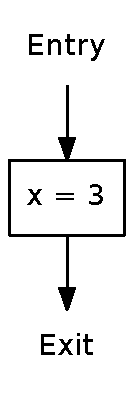
\includegraphics[scale=0.4]{figures/simple.pdf}
    \caption{A single statement}
  \end{subfigure}
  ~
  \begin{subfigure}[b]{0.49\textwidth}
    \center
    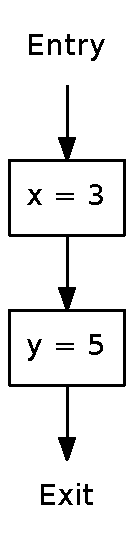
\includegraphics[scale=0.4]{figures/sequence.pdf}
    \caption{A sequence of two statements}
  \end{subfigure}
  \caption{Construction of a control flow graph for two sequential statements}
  \label{cfg_sequence}
\end{figure}

The CFGs of  control flow structures in the Python programming language was presented in the figures provided in \cref{python:control_structures}.

\textbf{Note} that the \textit{else} clause is not represented as a independent node, the false branch is represented in the same way as the true branch in a ``if-else'' structure.
\todo{synes maske det skal flyttes til eksemplet, men det kommer an pa hvordan tekster i python eksemplet bliver}

The CFG for a complete program is produced by systematically combining the building blocks.
A CFG of the general example in \cref{theory:general_code_example}, is shown on \cref{theory:general_code_example_cfg}.

\begin{figure}
  \center
  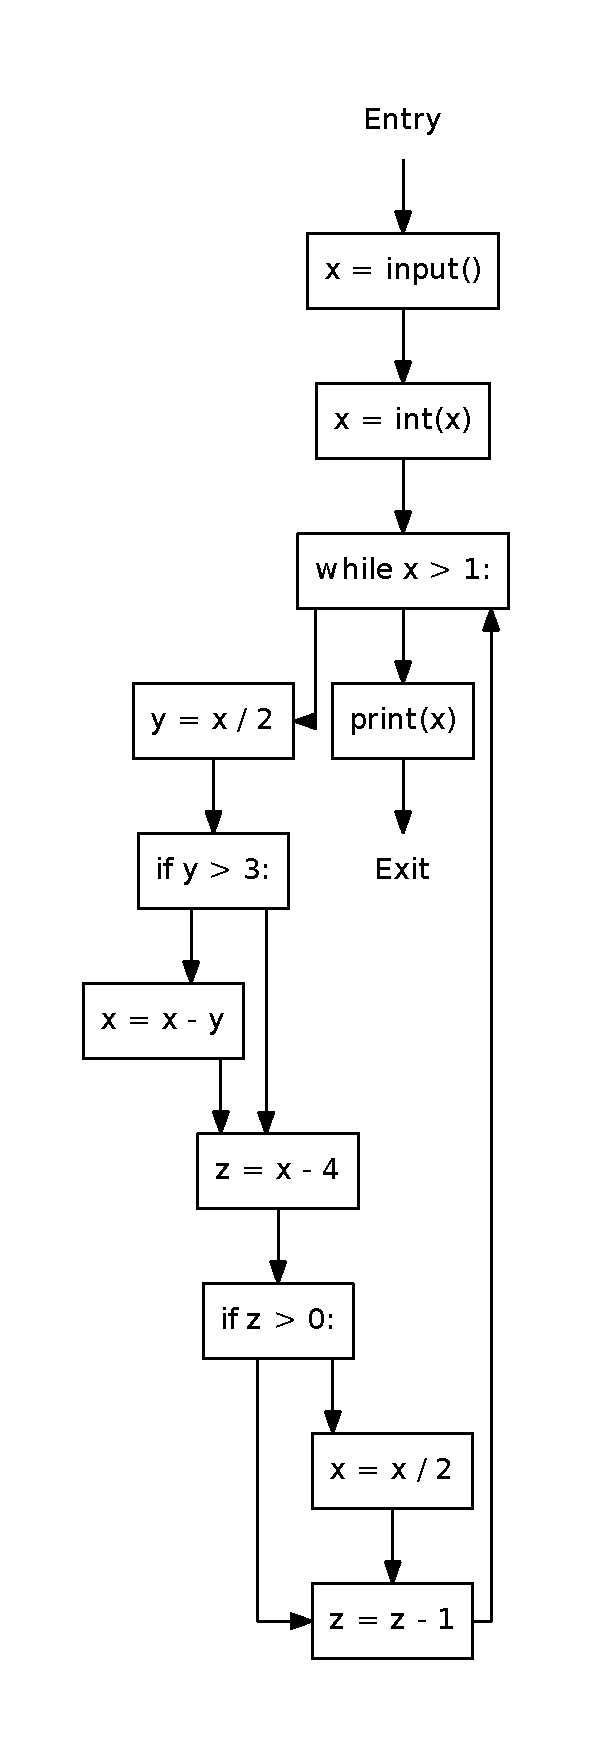
\includegraphics[width=.25\textwidth]{figures/general_example.pdf}
  \caption{The control flow graph of the general example, \cref{theory:general_code_example}.}
  \label{theory:general_code_example_cfg}
\end{figure}

\section{Interprocedural analysis}
As Python contain functions we need a strategy for dealing with these.
One strategy is to handle each function individually.
This strategy requires that we assume the worst about every function call, because we cannot know that it should not be the case.

The alternative is called interprocedural analysis, and produces a single CFG from a program with a number of function calls.
This is done by \emph{gluing} the function bodies into the main CFG every time a function is called.


On \cref{interprocedural_cfgs} is an example of two CFGs where the first one calls a function, which is represented by the second CFG.
The analysis need to be able to glue these together without changing the semantics of the program.

\begin{figure}[H]
  \center
  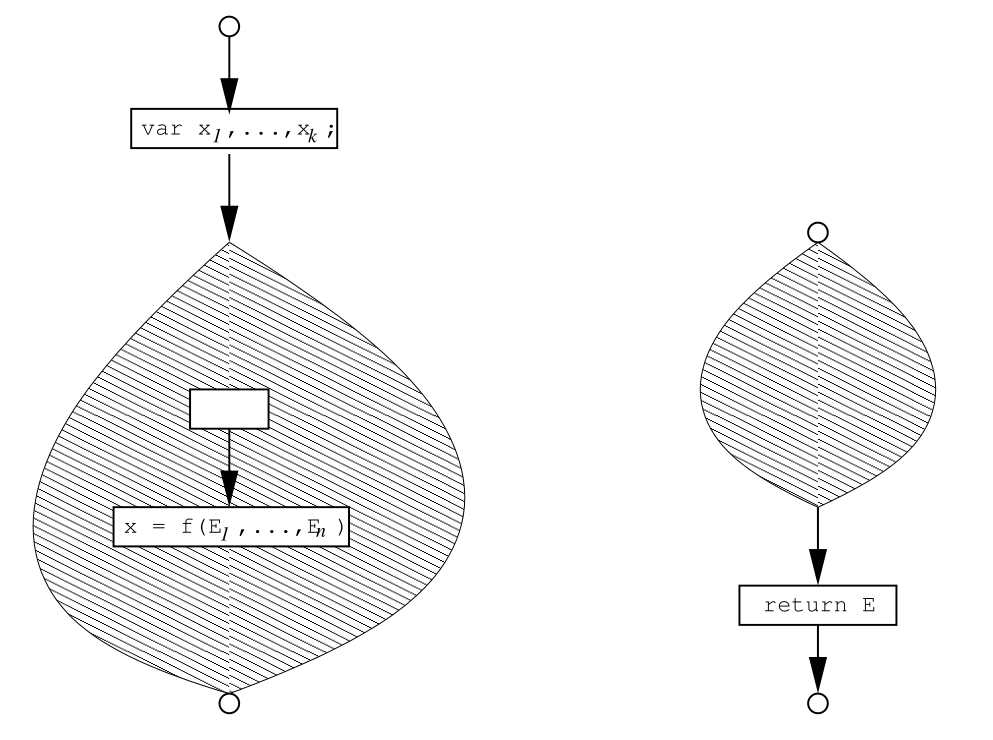
\includegraphics[width=0.6\textwidth]{figures/interprocedural_cfgs}
  \caption{Two CFGs, one for the calling function and one for the called function}
  \label{interprocedural_cfgs}
\end{figure}


\paragraph{Shadow variables}
In order to maintain the correct values for all variables across scopes we introduce \emph{shadow variables}.
Because parameters of functions have no relation to the scope of other functions, parameters can be the same for many different function scopes.
Shadow variables ensure that the meaning of the different scopes are kept when gluing the function CFG into the main CFG.
The process of gluing a function into the calling function can be split up into four steps:
\begin{itemize}
\item When calling a function we need to save the variables of the current scope, ensuring no clashes with the variabels of the function body.
\item Then we need to save all the formal parameters of the function definition and insert the actual parameters into the appropriate variables in order to create the function local scope.
\item The body of the function can now be inserted as it was originally defined, with the exception that all returns need to be assigned to a unique variable.
\item After the function body all the saved variables need to be restored.
\end{itemize}

The final result is a single CFG for the caller with the callee interwoven in.
The result is depicted on \cref{interprocedural_glue}.
Here all the saved variables are characterized with a prefix and a number \emph{i}, which is a unique index for the called function.


\begin{figure}[H]
  \center
  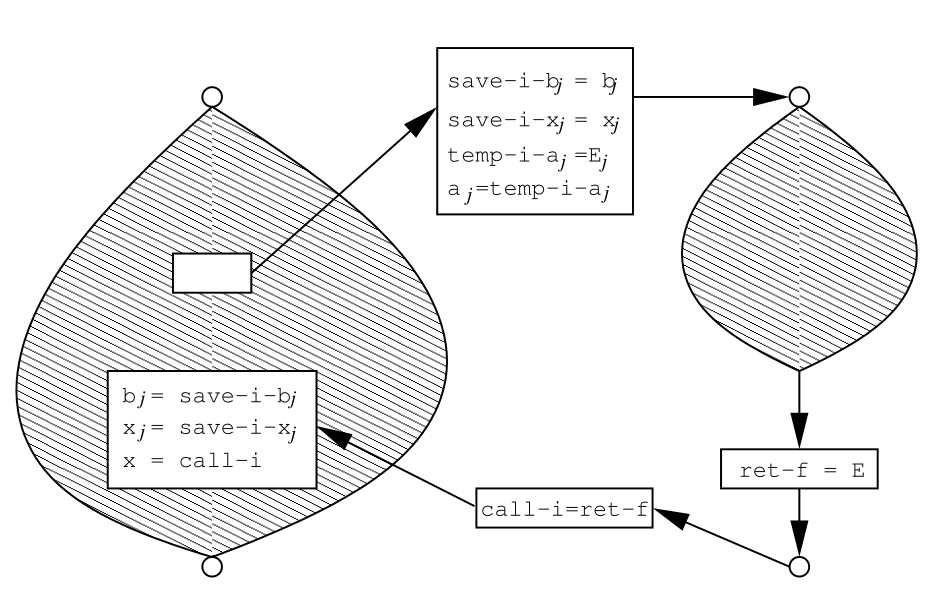
\includegraphics[width=0.6\textwidth]{figures/interprocedural_glue}
  \caption{The two CFGs glued together with shadow variables}
  \label{interprocedural_glue}
\end{figure}

\paragraph{Polyvariance}
If we ``glue in'' the function bodies of called function by referencing the respective CFG, we get a \emph{monovariant} analysis.
An example of monovariant analysis can be seen on \cref{monovariant}
This method has puts some limitiations on the analyses that are performed on the CFG.
For example constant propagation analysis will be inaccurate because more than one call will be represented in the callee CFG.
For our purposes we need propagation of assignments to be accurate for an arbitrary number of calls to a function.

The solution is to make the analysis \emph{polyvariant}.
This is done by make multiple copies of the function body for each call site.
This solves the problem about propagation because every call site has a separate copy of the function where the analysis can perform unique calculations.

\begin{figure}[H]

  \begin{subfigure}[b]{0.49\textwidth}
    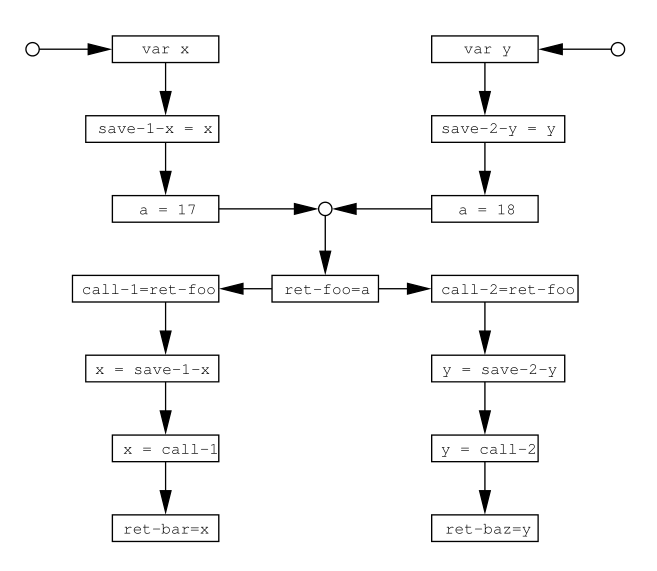
\includegraphics[width=\textwidth]{figures/monovariant}
    \caption{Example CFG of monovariant analysis}
    \label{monovariant}
  \end{subfigure}
 ~ 
  \begin{subfigure}[b]{0.49\textwidth}
    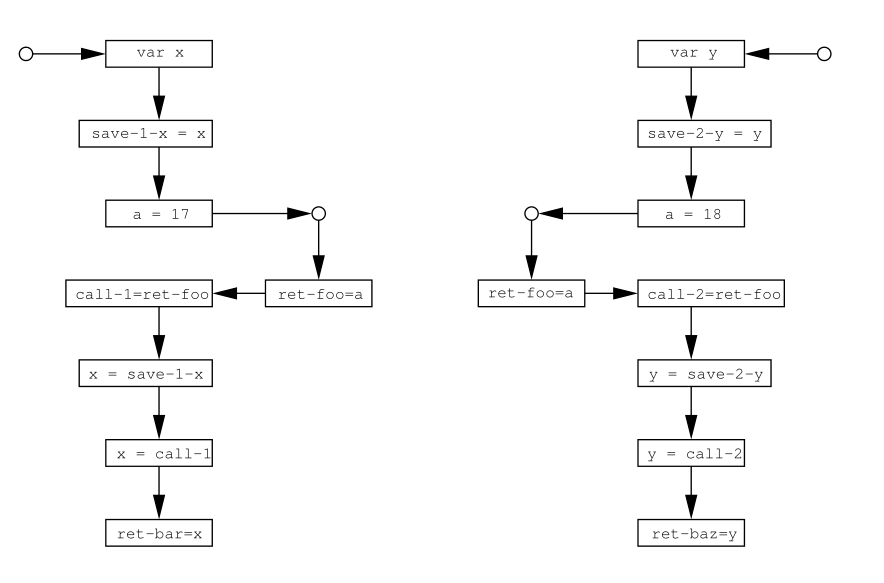
\includegraphics[width=\textwidth]{figures/polyvariant}
    \caption{Example CFG of polyvariant analysis}
    \label{polyvariant}
  \end{subfigure}
  
  \caption{The difference betweem monovariant and polyvariant interprocedural analysis}
  \label{monopoly}
\end{figure}
\todo{the figures use var, do we edit them, footnote or something else?}

\todo{python call by assignment?}

\section{Lattice Theory}
  The static analysis we want to perform utilizes the mathematical theory of lattices together with a monotone function to guarantee that the analysis will terminate.

  \paragraph{Partial orders}
  A lattice is a specialization of a partial order which will be described.
  A partial order is a mathematical structure $L = (S, \sqsubseteq)$

\section{Monotone functions}
A function $f: L \to L$ is monotone when $\forall x,y \in S : x \sqsubseteq y \Rightarrow f(x) \sqsubseteq f(y)$.
Being monotone does not imply that the function is increasing.
All constant functions are monotone.

If we look at the least upper bound and greatest lower bound functions they are monotone in both arguments.
This means that we can apply the least upper bound function on two arguments and be certain that it will never decrease.
This is an important requirement for the fixed-point theorem which will be presented in the next section.

\section{Monotone functions}
A function $f: L \to L$ is monotone when $\forall x,y \in S : x \sqsubseteq y \Rightarrow f(x) \sqsubseteq f(y)$.
Being monotone does not imply that the function is increasing.
All constant functions are monotone.

If we look at the least upper bound and greatest lower bound functions they are monotone in both arguments.
This means that we can apply the least upper bound function on two arguments and be certain that it will never decrease.
This is an important reqiurement for the fixed-point theorem which will be presented in the next section.

\section{Fixed-point}
For the static analysis of a program we need a theorem that can find the best approximation of some dataflow problem.
Because we will generally consider problems that are undecidable, see \cref{theory_intro}, we need a framework that overestimate the answer, and thus makes an approximation.

This framework will be based on the fixed-points theorem which states the following (quoted from \citet[p.~13]{schwartzbach}):

\begin{definition}{Fixed-point theorem}
In a lattice L with finite height, every monotone function $f$ has a unique least fixed-point defined as
\[ fix(f) = \bigsqcup_{i \ge 0} f^i(\bot) \]

for which $f(fix(f)) = fix(f)$
\end{definition}

\noindent
The proof of this theorem can be found in \citep[p.~13]{schwartzbach}.

This theorem enables us to find an approximation to an undecidable problem by walking up the lattice until a fixed-point is reached.
This computation has been illustrated in \cref{lattice_walk} where the analysis starts at $\bot$ and end in the fixed-point which is the approximation to the problem at hand.

\begin{figure}
\begin{center}
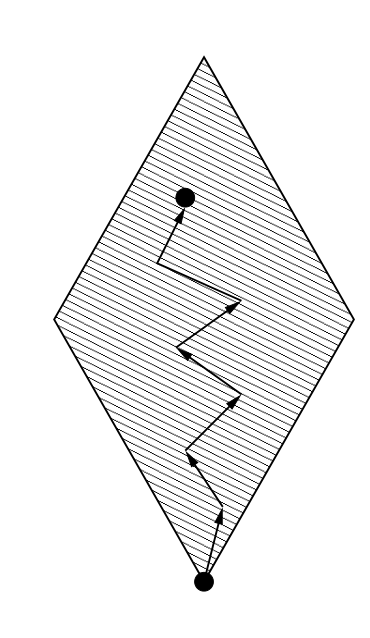
\includegraphics[width=0.2\textwidth]{figures/fixed-point_walk}
\end{center}
\caption{A walk through the lattice, starting a $\bot$ and ending in the fixed-point}
\label{lattice_walk}
\end{figure}

\section{Systems of Equations}\label{theory:fixedpoint:systemsofequations}
Combining equations into a system of equations can be solved by using fixed-points.
Consider an equation system of the form:

$
\begin{array}{l c l}
x_1 = F_1(x_1, \dots, x_n) \\
x_2 = F_2(x_1, \dots, x_n)\\
\vdots\\
x_n = F_n(x_1, \dots, x_n)\\
\end{array}
$

Here $x_i$ are variables and $F_i: L^n \rightarrow L$ is a monotone function.
A least unique solution to such a system can be found as the least fixed-point of the combined function $F : L^n \rightarrow L^n$ defined by:

$F(x_1, \dots, x_n) = (F_1(x_1, \dots, x_n), \dots, F_n(x_1, \dots, x_n)) $

\section{Systems of Equations}\label{theory:fixedpoint:systemsofequations}
Combining equations into a system of equations can be solved by using fixed-points.
Consider an equation system of the form:

$
\begin{array}{l c l}
x_1 = F_1(x_1, \dots, x_n) \\
x_2 = F_2(x_1, \dots, x_n)\\
\vdots\\
x_n = F_n(x_1, \dots, x_n)\\
\end{array}
$

Here $x_i$ are variables and $F_i: L^n \rightarrow L$ is a monotone function.
A least unique solution to such a system can be found as the least fixed-point of the combined function $F : L^n \rightarrow L^n$ defined by:

$F(x_1, \dots, x_n) = (F_1(x_1, \dots, x_n), \dots, F_n(x_1, \dots, x_n)) $

\section{Dataflow Constraints}
For analysing a CFG of a program we need to be able to describe the relationship between the individual nodes.
Some analyses track variable content while others track use of certain expressions.
Similarly, some analyses need information from its successors while others need information from its predecessors.

To describe these different analyses we annotate each node with a \emph{dataflow constraint}.
Dataflow constraints relate the value of a node to its neighboring nodes and is denoted $\constraint{v}$.
A dataflow analysis consists of a number of dataflow constraints that each defines the relation of a construction in the programming language.

An example of a dataflow constraint could be conditions (from the liveness example in \citet{schwartzbach})
\[ \constraint{v} = JOIN(v) \cup vars(E) \]

where JOIN combines the constraints of the successors of $v$ and vars(E) denote the set of variables occuring in E.

\section{The Fixed-point Algorithm}\label{fixed_point_algorithm}
A CFG has been defined in \cref{control_flow_graph} and a lattice has been defined in \cref{lattice}.
Given a CFG and lattice a fixed-point algorithm can be defined.
The following is from \citet{schwartzbach}.


Operating on a CFG that contains the nodes $\{ v_1, v_2, \dots, v_n \}$ we work with the lattice $L^n$.
Assuming that the node $v_i$ generates the dataflow equation $\llbracket v_i \rrbracket = F_i ( \llbracket v_1 \rrbracket, \dots, \llbracket v_n \rrbracket)$, the equations of all the nodes can be combined in a function $ F: L^n \rightarrow L^n$.

\[ F(x_1, \dots, x_n) = (F_1(x_1, \dots, x_n), \dots, F_n(x_1, \dots, x_n)) \]

This combined function resembles the function presented in \cref{theory:fixedpoint:systemsofequations}, and it can indeed be solved by fixed-points.
A naive algorithm for solving such a function is presented in \citet{schwartzbach}:

\begin{algorithmic}
  \State $x = (\bot, \dots, \bot)$
  \Do
  \State $t = x$
  \State $x = F(x)$
  \doWhile $ x \ne t $
\end{algorithmic}

\todo{if we use the more advanced algorithms, write them here}

\section{Dataflow analysis}
The type of dataflow analysis that we want to perform is called the \emph{monotone framework}.
The monotone framework utilizes the concepts that have now been introduced.

A CFG of the program is generated to represent the flow of the program.
A lattice with finite height together with a collection of dataflow constraints comprise the analysis to be performed.
Running the fixed-point algorithm on the parts will result in an approximation of the answer to the analysis which can then be interpreted.



\subsection{Reaching definitions}
To solve our problem of detecting when unsanizited user input reaches a critical point in the code, we need an analysis of what assignments may influence the values of all variables at any point in the program.
The \emph{Reaching Definitions} as presented in \citet[p.~26]{schwartzbach} achieves just this.

Consider the following python code (the example corresponds to the examples in \citet{schwartzbach} adapted to runnable python code):
\begin{lstlisting}[numbers=left, frame=single, linewidth=6cm]
x = input()
x = int(x)
while x > 1:
    y = x / 2
    if y > 3:
        x = x-y
    z = x-4
    if z > 0:
        x = x / 2
    z = z - 1
print(x)
\end{lstlisting}

The code is very simple, it take some user input which is sent through a while loop that changes the three variables x,y and z.
The x variable is printed out as the last operation of the program.
At this point x has been changed by assignments a number of times, and it is not obvious where the value comes from.
By performing the reaching definitions analysis we can find possible origins of the value.

\paragraph{Performing the analysis}
As stated earlier a dataflow analysis consist of many of the concepts that have been introduced until now.
These concepts will in the following be instantiated on the previously introduced example as to present the complete analysis.

\subparagraph{Control flow graph}
The CFG of this code is presented in \cref{reaching::cfg}.

\begin{figure}
  \begin{center}
  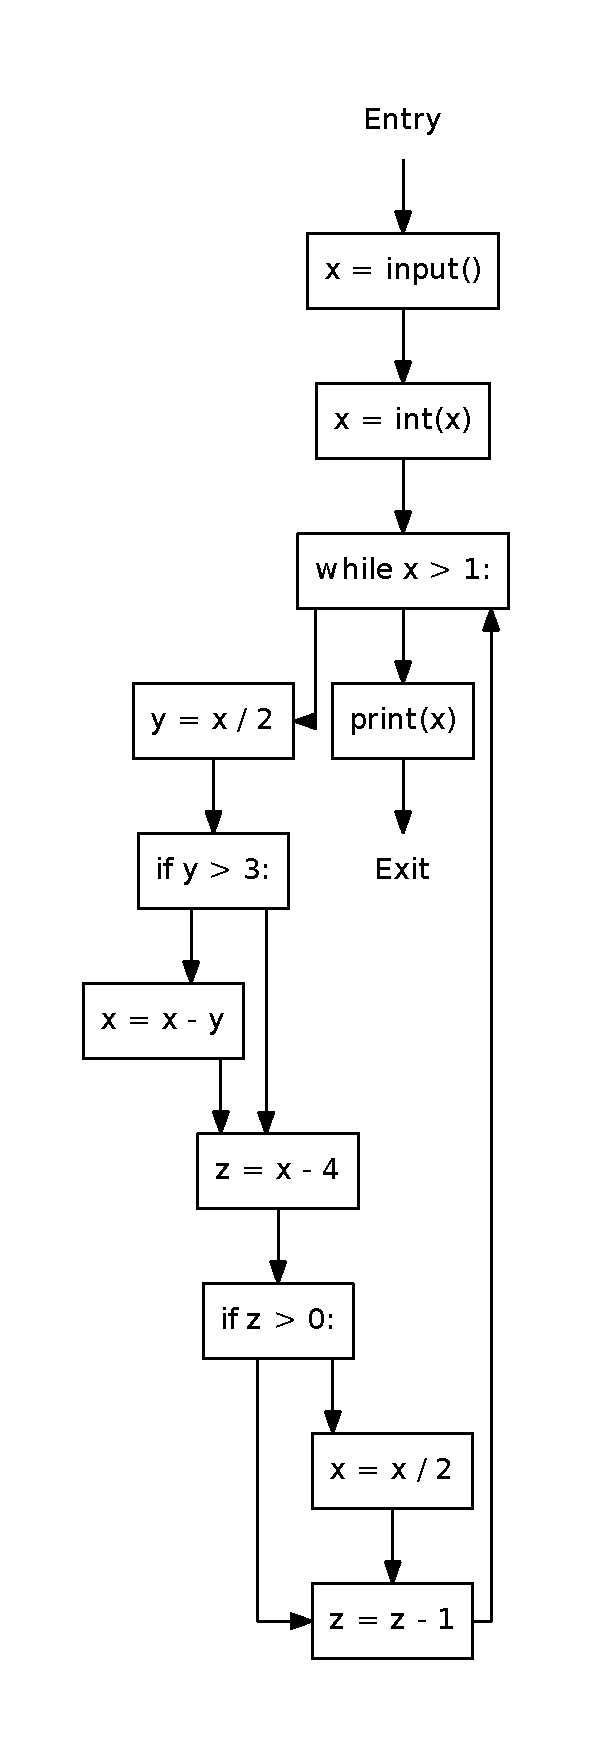
\includegraphics[scale=.5]{./figures/reaching_definitions.pdf}
  \caption{CFG of the python code presented in \cref{reaching::code}}
  \label{reaching::cfg}
  \end{center}
\end{figure}


\subparagraph{Lattice}
The lattice used for this analysis is a powerset lattice of all the assignments in the program.

\[ L = ( 2^{ \{x = \text{input()}, ~ x = \text{int(x)}, ~ y = x/2, ~ x = x-y, ~ z = x-4, ~ x = x/2, ~ z = z-1 \} } , \subseteq ) \]

\todo{visualization of the lattice - do this or not?}

\subparagraph{Dataflow Constraint System}
The analysis is performed backwards by joining the constraints of all predecessors of all nodes.
This can be expressed a the following function:

\[ JOIN(v) = \bigcup_{ w \in pred(v)} \constraint{w} \]

All nodes other that assignment just join all constraints of their predecessors:

\[ \constraint{v} = JOIN(v) \]

Assignment nodes changes the content of a variable and the former assignment to this variable will therefore be discarded:

\[ \constraint{v} = JOIN(v) \downarrow id \cup \{ v \} \]

Where the $\downarrow$ function removes all assignements to the variable $id$ from the result of the JOIN.

Applying the previously defined dataflow constraints to the generated CFG looks as follows:

\begin{figure}[H]
\[
\begin{array}{l}
  \constraint{entry} = \{\}\\
  \constraint{x = input()} = \assignconstraint{\constraint{entry}}{x}{x = input()}\\
  \constraint{x = int(x)} = \assignconstraint{\constraint{x = input}}{x}{x = int(x)}\\
  \constraint{\text{while } x > 1} = \constraint{x = int(x)} ~ \cup ~ \constraint{z = z - 1}\\
  \constraint{ y = x / 2} = \assignconstraint{\constraint{\text{while } x > 1}}{y}{y = x / 2}\\
  \constraint{\text{if } y > 3} = \constraint{ y = x / 2}\\
  \constraint{ x = x-y} = \assignconstraint{\constraint{\text{if } y > 3}}{x}{x = x-y}\\
  \constraint{ z = x-4} = \assignconstraint{(\constraint{x = x-y} ~ \cup ~ \constraint{\text{if } y > 3})}{z}{z = x-4}\\
  \constraint{\text{if } z > 0} = \constraint{z = x - 4}\\
  \constraint{x = x / 2} = \assignconstraint{\constraint{\text{if } z > 0}}{x}{x = x/2}\\
  \constraint{z = z - 1} = \assignconstraint{(\constraint{\text{if } z > 0} ~ \cup ~ \constraint{x = x / 2}}{z}{z = z - 1}\\
  \constraint{print(x)} = \constraint{\text{while } x > 1}\\
  \constraint{exit} = \constraint{print(x)}
\end{array}
\]
\caption{Dataflow constraints applied on the generated CFG}
\end{figure}

\paragraph{Solving the equation system}
Solving this system of equations with the fixed-point algorithm will provide the information we need in order work with our problem.

The first iteration of this looks as follows:

\begin{figure}[H]
\[
\begin{array}{l}
  \constraint{entry} = \{\}\\
  \constraint{x = input()} = \{x = input()\}\\
  \constraint{x = int(x)} = \{x = int(x)\}\\
  \constraint{\text{while } x > 1} = \{\}\\
  \constraint{ y = x / 2} = \{ y = x / 2\}\\
  \constraint{\text{if } y > 3} = \{\}\\
  \constraint{ x = x-y} = \{ x = x - y \} \\
  \constraint{ z = x-4} = \{z = x-4 \} \\
  \constraint{\text{if } z > 0} = \{\}\\
  \constraint{x = x / 2} = \{ x = x / 2 \}\\
  \constraint{z = z - 1} = \{ z = z -1 \} \\
  \constraint{print(x)} = \{\}\\
  \constraint{exit} = \{\}\\
\end{array}
\]
\caption{First iteration of the fixed-point algorithm}
\label{reachingdefinitions:firstiteration}
\end{figure}

Here it is clear that only the constraints of assignments have walked up the lattice, each to the node indicating the flownode itself.
After nine iterations all the assignments will propagate through the program, and the result can be seen on \cref{reachingdefinitions:finaliteration}.
These constraints can now be interpreted in order to answer question that require knowledge of which assignments reach which nodes.

\begin{figure}[H]
\[
\begin{array}{l}
  \constraint{entry} = \{\}\\
  \constraint{x = input()} = \{x = input()\}\\
  \constraint{x = int(x)} = \{x = int(x)\}\\
  \constraint{\text{while } x > 1} = \{ x = int(x), ~ y = x / 2, ~ x=x-y, ~ x = x/2, ~ z=z-1 \}\\
  \constraint{ y = x / 2} =  \{ x = int(x), ~ y = x / 2, ~ x=x-y, ~ x = x/2, ~ z=z-1 \}\\
  \constraint{\text{if } y > 3} =  \{ x = int(x), ~ y = x / 2, ~ x=x-y, ~ x = x/2, ~ z=z-1 \}\\
  \constraint{ x = x-y} =  \{ y = x / 2, ~ x=x-y, ~ z=z-1 \}\\
  \constraint{ z = x-4} =  \{ x = int(x), ~ y = x / 2, ~ x=x-y, ~ z=x-4, ~ x = x/2\}\\
  \constraint{\text{if } z > 0} = \{ x = int(x), ~ y = x / 2, ~ x=x-y, ~ z=x-4, ~ x = x/2\}\\
  \constraint{x = x / 2} = \{ y = x / 2, ~ z=x-4, ~ x = x/2\}\\
  \constraint{z = z - 1} = \{ x = int(x), ~ y = x / 2, ~ x=x-y, ~ x = x/2, ~ z=z-1 \}\\
  \constraint{print(x)} = \{ x = int(x), ~ y = x / 2, ~ x=x-y, ~ x = x/2, ~ z=z-1 \}\\
  \constraint{exit} = \{ x = int(x), ~ y = x / 2, ~ x=x-y, ~ x = x/2, ~ z=z-1 \}\\
\end{array}
\]
\caption{Final result of the fixed-point algorithm}
\label{reachingdefinitions:finaliteration}
\end{figure}

\paragraph{Interpreting the result}

Looking at the final equations the potential flow of values through the program can be seen.
For exampel, looking at the print statement, the value of x could have originated from three places in the program: the $x = int(x)$, $x = x-y$ or the $x = x/2$ statement.
Depending on the purpose of the analysis, this information can be used to deduce whether any dangerous flows are possible.

\section{Taint Analysis}
The following is based on \citet[Part 3]{schwartz2010all}.
Taint analysis is used for tracking the information between sources and sinks.
If some data comes from an untrusted or tainted source it is a tainted.
All other data is untainted.
Which sources introduce taint are defined by the user of the analysis.

If a taint analysis is marking too much data as taint it is called \textit{overtainting}.
If a taint analysis is marking too little data as taint it is called \textit{undertainting}.
If the analysis is \textit{precise} it means there is no over- or undertainting.
Undertainting leads to missing some vulnerabilities and overtainting leads to having some false positive vulnerabilities.

Because finding all vulnerabilities is critical it is common to use the approach of overtainting.
This can lead to a problem called \textit{taintspread} which is when more and more data is tainted and that with less precision.
To help with that, one can use \textit{sanitisers} to untaint data.

\section{Analysis extension}
The previously described algorithm is able to detect that a value flows from a source to a sink.
Unfortunately this method is insufficient in finding all vulnerabilities.
When a value from a source is assigned to a variable \textit{s}, this variable is not necessarily the one being used when arriving at a sink.
Other variables can be assigned to values that derive from \textit{s}, or \textit{s} can be reassigned to a modified version of \textit{s}.

These two problems arise from using the method presented in \cref{theory:reaching}.
Two small examples of the problems can be seen in \cref{ext:reassign} and \cref{ext:assign}.
Here the method \texttt{source} is an arbitrary method that introduces taint while \texttt{sink} is an arbitrary sensitive sink.

\begin{figure}[h]

  \begin{subfigure}[b]{0.45\textwidth}
    \begin{lstlisting}[style=python]
s = source()

s = 'input: ' + s

sink(s)
    \end{lstlisting}
    \caption{Reassigning a tainted variable with a modification of the tainted value}
    \label{ext:reassign}
  \end{subfigure}
  ~~
  \begin{subfigure}[b]{0.45\textwidth}
    \begin{lstlisting}[style=python, numbers=none]
s = source()

user_input = 'input: ' + s

sink(user_input)
    \end{lstlisting}
    \caption{Assigning a derived value of the tainted variable}
    \label{ext:assign}
  \end{subfigure}
\end{figure}

In neither of the two examples it will be possible to detect the vulnerability with the method from \cref{theory:reaching}, because the flow is cut off by the assignments.
To fix this we have introduced two extensions to the method.

\subsection{Propagation of reassignments}
In order to maintain the tainted variable \textit{s} 'alive' we have modified the assignment dataflow constraint presented in \cref{theory:reaching}.
We want to let both the original assignment as well as the reassignment live in the analysis.
First we check if the current assignment is a reassignment.
An assignment is a reassignment if the variable assigned to also is part of the right hand side.
If it is a reassignment, we omit the arrow function of the original rule, else the rule is as defined originally.
The extended constraint rule is shown below:

\begin{align*}
  \constraint{v} = &\text{ if v is a reassignment:}\\
  &\phantom{==}JOIN(v) \cup \{ v \}\\
  &\text{ else:}\\
  &\phantom{==}JOIN(v) \downarrow id \cup \{ v \}\\
\end{align*}

Now both the original assignment and the reassignment will propagate to the sink.

\subsection{Assignment of Variable derivations}\label{ext:derivation}
To be able to detect derivatons of variables as being vulnerabilities, we need to keep track of assignments to these derivations.
This will be done when finding sources in the CFG.
Each time a source is found, the subsequent nodes will be checked for assignments of derivations of this source node.
Nodes that fit this description will be saved together with the source node as a 'secondary' source node.
When checking for pairs of sources and sinks these assignments will also be considered as sources.

\section{Finding vulnerabilities}\label{theory_finding_vulns}
Armed with the information provided by the reaching definitions analysis we should be able to find vulnerabilities in applications.
The vulnerabilities mentioned in \cref{security_vulnerabilities} all have in common that one expression introduces user input into the program, and a later expression executes this input.
The structure of such application is outlined on \cref{vulnerabilities_unsanitised}.
Untrusted user input is denoted as a \emph{source}, while a piece of sensitive code is denoted as a \emph{sink}.

Using the reaching definitions analysis it is possible to determine if the data obtained at the source will reach the sink, by examining the constraints provided by the analysis.
The secondary nodes mentioned in \cref{ext:derivation} will likewise be considered as a source.
If the source is contained in the set of constraints of the sink and the source variable is being used as a parameter by the sink, we can regard it as a potential security vulnerability.

Such a vulnerability can potentially be harmless because of processing on the path towards the sink.
A function that takes some untrusted input and returns a harmless version will be denoted as a \emph{sanitiser}.
\Cref{vulnerabilities_sanitised} shows the outline of an application with a sanitiser.
The flow of such a program makes it impossible to guarantee that the application is safe, but reporting it to the developer may ease the process of securing the application.

\begin{figure}
  \begin{subfigure}[b]{0.5\textwidth}
    \centering
    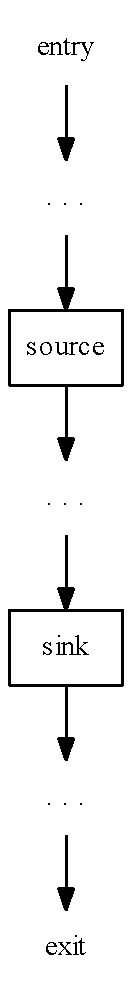
\includegraphics[scale=0.8]{figures/dot_files/unsanitised.pdf}
    \caption{A vulnerable application}\label{vulnerabilities_unsanitised}
  \end{subfigure}
  ~
  \begin{subfigure}[b]{0.5\textwidth}
    \centering
    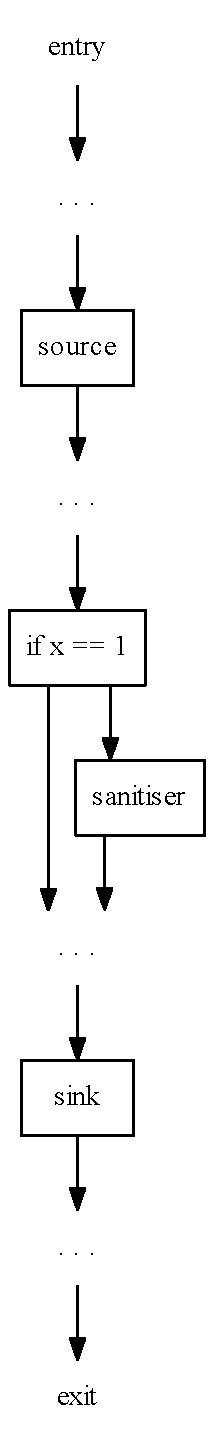
\includegraphics[scale=0.8]{figures/dot_files/sanitised_with_flow.pdf}
    \caption{A sanitiser eliminating the vulnerability}
    \label{vulnerabilities_sanitised}
  \end{subfigure}
  
  \caption{Control Flow Graphs for applications with potential vulnerabilities}
\end{figure}
\todo{draft, vi skal nok overveje denne sektion igen når vi har alle detaljer omkring taint, propagation og sanitiser handling på plads}


\chapter{Implementation}
\section{Implementation Overview}
This section will give an overview of the different components and the overall flow of \pyt{}.
An illustration giving an abstract overview can be seen on \cref{figure:implementation_overview}.

\begin{figure}
  \begin{tikzpicture}
\newcommand\XLabel{7}
\newcommand\XNode{10}
\newcommand\XEngines{14}
\newcommand\TextWidth{3}
\tikzset{>=latex}

%\draw[help lines] (5,5) grid (15,20);

%%%%%%%%%%%% MID STRUCTURE %%%%%%%%%%%%%%%%%%%
\node[inner sep=10pt] (code) at (\XNode,18)
    {
\includegraphics[width=.1\textwidth]{./figures/dot_files/implementation_overview_images/source_code.png}};
\node[text width=\TextWidth{}cm] at (\XLabel,18) {\hfill{}Source code};

\node[inner sep=10pt] (ast) at (\XNode,15)
    {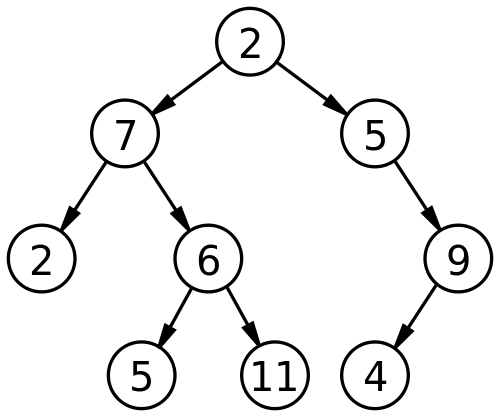
\includegraphics[width=.15\textwidth]{./figures/dot_files/implementation_overview_images/ast.png}};
\node[text width=\TextWidth{}cm] at (\XLabel,15) {\hfill{}AST};

\node[inner sep=10pt] (cfg) at (\XNode,11)
    {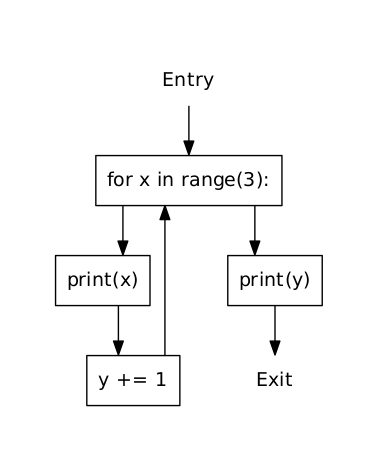
\includegraphics[width=.2\textwidth]{./figures/dot_files/implementation_overview_images/for_complete.png}};
\node[text width=\TextWidth{}cm] at (\XLabel,11) {\hfill{}CFG};

\node[inner sep=10pt] (engine) at (\XNode,7)
    {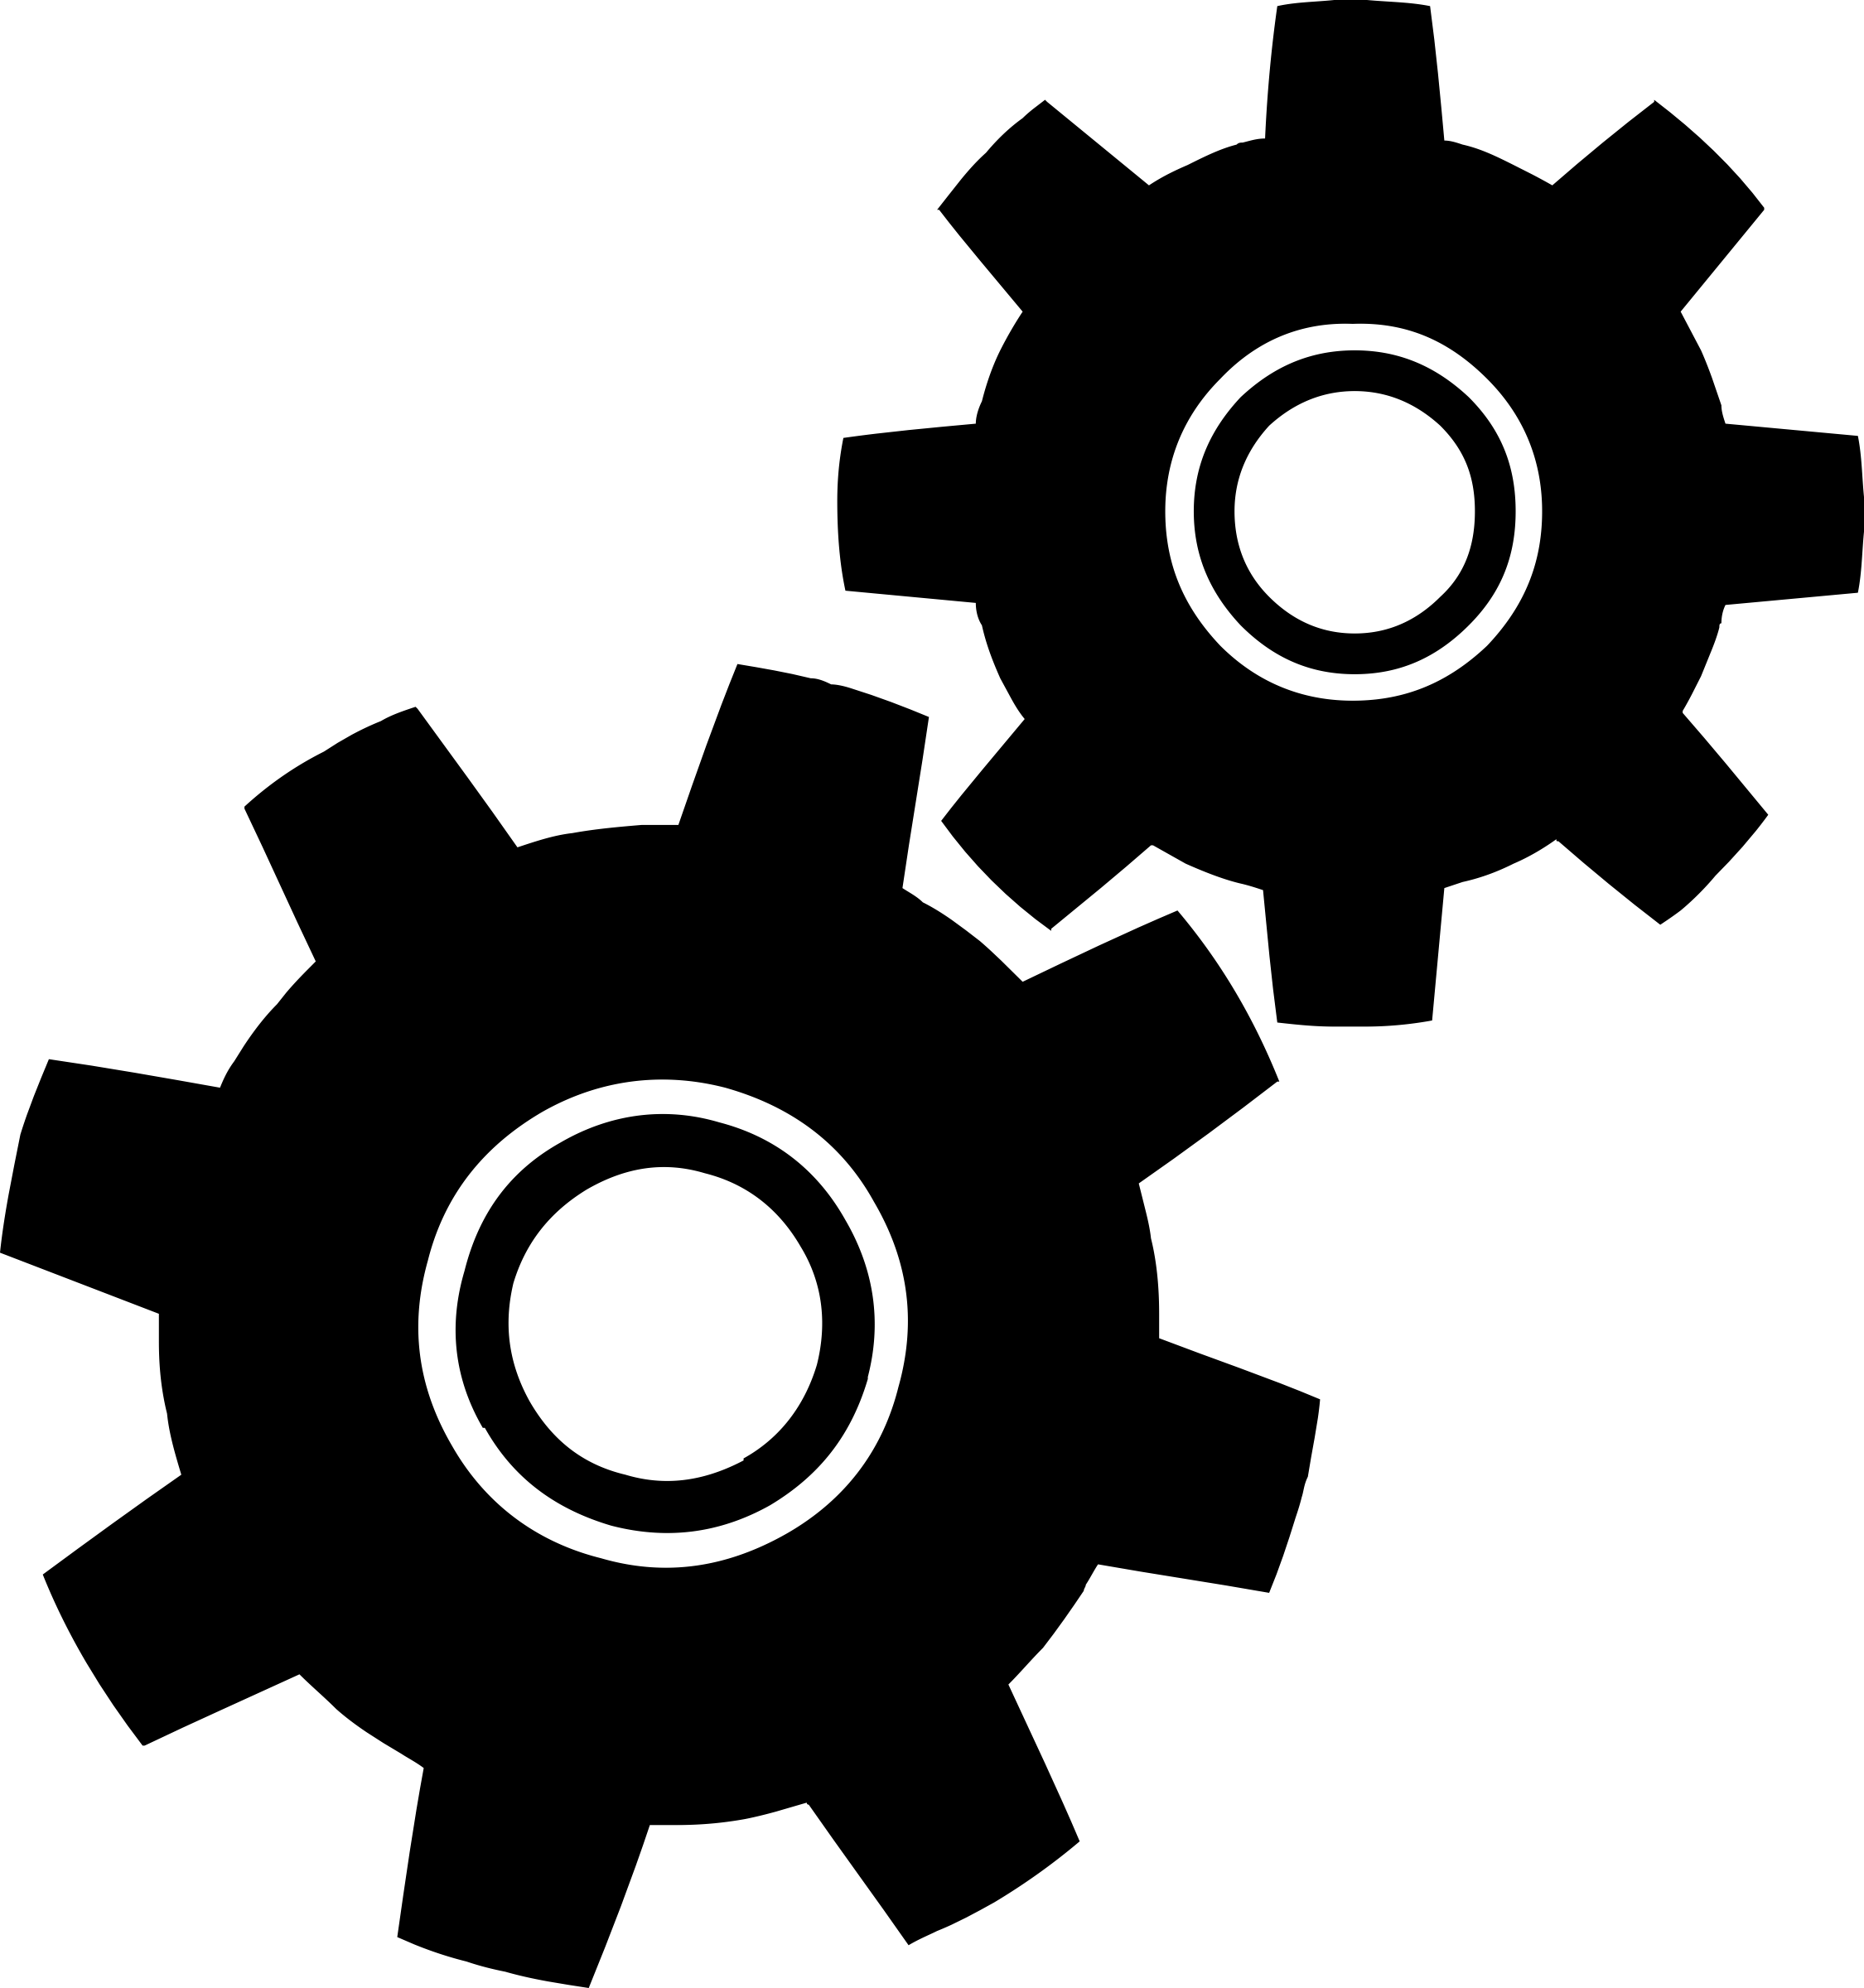
\includegraphics[width=.1\textwidth]{./figures/dot_files/implementation_overview_images/cog_wheel.png}};
\node[text width=\TextWidth{}cm] at (\XLabel,7) {\hfill{}Engine};

\node[inner sep=10pt] (algorithm) at (\XNode,4)
    {
\includegraphics[width=.1\textwidth]{./figures/dot_files/implementation_overview_images/spiral.png}};
\node[text width=\TextWidth{}cm] at (\XLabel,4) {\hfill{}Fixed Point \\ \hfill{}Algorithm};

\node[inner sep=10pt] (vulnerabilities) at (\XNode,1)
    {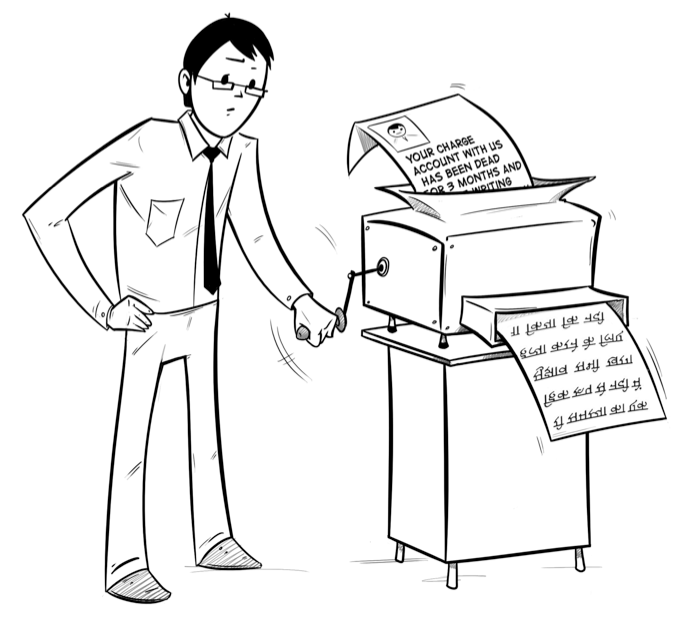
\includegraphics[width=.15\textwidth]{./figures/dot_files/implementation_overview_images/vulnerability.png}};
\node[text width=\TextWidth{}cm] at (\XLabel,1) {\hfill{}Vulnerabilities};

%%%%%%%%%%%%%%%%%%%% ENGINES %%%%%%%%%%%%%%%%%%%%%%%%
\node[inner sep=10pt] (flask) at (\XEngines,11)
    {
\includegraphics[width=.2\textwidth]{./figures/dot_files/implementation_overview_images/flask_text.png}};

\node[inner sep=5pt] (django) at (\XEngines,9)
    {
\includegraphics[width=.13\textwidth]{./figures/dot_files/implementation_overview_images/django.png}};

\node[label=below:{Other}, inner sep=5pt] (other_engine) at (\XEngines,7)
    {
\includegraphics[width=.05\textwidth]{./figures/dot_files/implementation_overview_images/question_mark.png}};

%%%%%%%%%%%%%%%% ANALYSIS %%%%%%%%%%%%%%%%%%%%%%%%%    
\node[label=below:{Analysis}, inner sep=10pt] (analysis) at (\XEngines,4)
    {
\includegraphics[width=.1\textwidth]{./figures/dot_files/implementation_overview_images/analysis.png}};

\node[text width=2cm, inner sep=10pt] (reaching) at (18,7) {Reaching Definitions};
\node[text width=2cm, inner sep=10pt] (liveness) at (18,4) {Liveness};

\node[label=below:{Other}, inner sep=5pt] (other_analysis) at (18,1)
    {
\includegraphics[width=.05\textwidth]{./figures/dot_files/implementation_overview_images/question_mark.png}};


\draw[->] (code) -- (ast);
\draw[->] (ast) -- (cfg);
\draw[->] (cfg) -- (engine);
\draw[->] (engine) -- (algorithm);
\draw[->] (algorithm) -- (vulnerabilities);

\draw[->] (flask) -- (engine);
\draw[->] (django) -- (engine);
\draw[->] (other_engine) -- (engine);

\draw[<->] (algorithm) -- (analysis);
\draw[->] (reaching) -- (analysis);
\draw[->] (liveness) -- (analysis);
\draw[->] (other_analysis) -- (analysis);

\end{tikzpicture}
  \caption{An abstract overview of the implementation of \pyt{}, showing the main components and the flow.}
  \label{figure:implementation_overview}
\end{figure}

The illustration shows that \pyt{} takes some source code as input and outputs at last a list of potential vulnerabilities.
After the source code is loaded an abstract syntax tree(AST) is generated.
The AST is generated using the standard Python library \texttt{ast}\cite{python_ast}.
One of the biggest components is the CFG component, which uses the AST nodes to make CFG nodes.
The engine is a component that uses a defined engine to prepare the CFG on the analysis.
The default engine is the Flask engine.
The fixed point algorithm is basically just implemented as the algorithm is described in \cref{fixed_point_algorithm}.
But it is able to use different analyses and as default it uses the reaching definitions analysis.
These analyses can be specified by the user.
At last a vulnerability log is provided to the user giving precise information about the potential vulnerabilities found.

\section{Handling Imports}
This section contains a rationale of how the imports are handled.
The two ways of importing files, import and import-from, are presented in \cref{python:import} and these two ways need to be handled separately.
The naming for import is prefixed by the name of the module while this is not the case for import-from.


The file that is given as input to \pyt{} is used as the entry point.
First of the \texttt{project\_handler} module is used to get local modules and project modules.
A local module is a Python file that is in the same folder as the file.
A project module is a Python file that is in the same project as the file.
The projects entry point is the folder the file is in or if another project root is specified.

To illustrate the above consider the following example project structure below.

\dirtree{%
.1 /.
.2 car\_app.
.3 app.py.
.3 models.py.
.3 user.
.4 forms.py.
.4 views.py.
}

So lets say that the entry point is the \textit{app.py} file.
This will result in a list of project modules containing the following modules: [\textit{car\_app.app.py, car\_app.models.py, car\_app.user.forms.py, car\_app.user.views.py}].
And a list of local modules containing the modules that are in the same folder as the entry file: [\textit{app.py, models.py}].


Using the \texttt{ast} module, described in \cref{library:ast}, the abstract syntax tree(AST) is generated for the entry point.
When visiting an import or import-from node the module and its definitions are loaded.
A definition in this context is a definition of a variable, function or class.

To illustrate consider these two modules:

\begin{lstlisting}[style=python, caption={A module that defines a function and two classes called \texttt{a}}, label={import:definition_module}]
  def fuel(km):
      ...

  class Car():
      ...

  class Owner():
      ...
\end{lstlisting}
\begin{lstlisting}[style=python, caption={A module called \texttt{b} importing the above module \texttt{a}}, label={import:import_module}]
  ...
  
  import a
  
  ...

  c = a.Car()
\end{lstlisting}

\todo{module definitions stakken kommer ud af ingenting her}

Looking at module \texttt{a} and \texttt{b} on \cref{import:definition_module} and \cref{import:import_module} respectively we will now see how the module definitions stack is built.
So first the AST for the entry file is created in this case we say its module \texttt{b}.
Then a module definitions is created for the current module.
So the stack contains one module definitions: stack = [module\_definitions<b>].

The AST is visited and when an import statement is visited a new module is visited and a new module definitions is created and added to the stack.
So we have the following stack: stack = [module\_definitions<b>, module\_definitions<a>]

The definitions in the import are: \texttt{foo}, \texttt{Car} and \texttt{Owner}.
These are added to the module definitions of module \texttt{a}: module\_definitions<a> = [\texttt{foo}, \texttt{Car}, \texttt{Owner}].
And to the  module definitions of module \texttt{b} which is accessed via the stack:  module\_definitions<b> = [\texttt{a.foo}, \texttt{a.Car}, \texttt{a.Owner}].

This is important so that when one of the imported definitions later is used the module definitions of module \texttt{a} does have knowledge about it.
Note that the names of the definitions are different.
This is because of the way the import statement works, see \cref{python:import}

Every time there is an import a new module definitions is created and added to the stack.
When the import is done the stack is popped.
This process handles the names for different modules and nested imports.

\section{Abstract Syntax Tree}
We use the built in python library \texttt{ast} for building an abstract syntax tree from the source code.
This module contains a \texttt{parse} method that constructs an AST from a string containing python code.
The abstract grammar of Python can be found in \cref{appendix:abstract_syntax}.
Selected rules, which are relevant for the following example, are displayed in \cref{ast_select_rules}.

\begin{lstlisting}[style=default, caption={Selected rules from the python abstract grammar}, label={ast_select_rules}]
mod = Module(stmt* body)

stmt = Assign(expr* targets, expr value)

expr = Num(object n)
     | Name(identifier id, expr_context ctx)
\end{lstlisting}

\Cref{ast_example} shows the abstract syntax tree for the small piece of code presented in \cref{ast_code}.
The root of the program is the \texttt{Module} statement which contains a list of \texttt{stmt}s.
In this case this \texttt{stmt} is an \texttt{Assign} which then contains a list of targets and a value.
In this concrete example there is a single target which is the \texttt{Name} x, and the value is a \texttt{Num} with the number 1.

\begin{figure}
  
  \begin{subfigure}[b]{0.5\textwidth}
    \begin{lstlisting}
      x = 1
    \end{lstlisting}
    \caption{A small python program}
    \label{ast_code}
  \end{subfigure}
  ~
  \begin{subfigure}[b]{0.5\textwidth}
    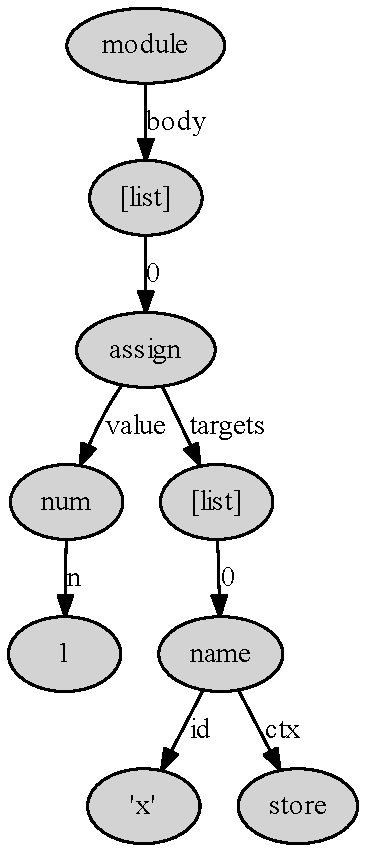
\includegraphics[scale=0.7]{figures/simple_ast.pdf}
    \caption{The syntax tree of the code in \cref{ast_code}}
  \end{subfigure}
  
  \caption{A piece of code and the corresponding syntax tree}
  \label{ast_example}
\end{figure}

\section{Control Flow Graph}
The \texttt{cfg} module contains a class, \texttt{Visitor}, that takes an AST and builds a CFG from it.
The CFG is built by traversing the generated AST using the visitor pattern.\cite{design_patterns}
The visitor pattern is implemented by the AST module, and our CFG module utilizes this implementation.
The \texttt{Visitor} class constructs a list of nodes which are saved as a \texttt{CFG}.

\begin{figure}[H]
  \begin{subfigure}[b]{0.2\textwidth}
    \begin{lstlisting}[style=python]
if True:
    x = 0
elif False:
    y = 0
else:
    z = 0
    \end{lstlisting}
    \caption{Code example}
    \label{CFG_if_code}
  \end{subfigure}
  ~~~ %add desired spacing between images, e. g. ~, \quad, \qquad, \hfill etc. 
  %(or a blank line to force the subfigure onto a new line)
  \begin{subfigure}[b]{0.4\textwidth}
    \begin{lstlisting}[style=default, basicstyle=\footnotesize, numbers=none]
If
   test
      NameConstant
   body
      [Assign]
   orelse
      If
         test
            NameConstant
         body
            [Assign]
         orelse
            [Assign]
    \end{lstlisting}
    \caption{Abstract Syntax Tree}
    \label{CFG_if_ast}
  \end{subfigure}
  ~
  \begin{subfigure}[b]{0.3\textwidth}
    \centering
    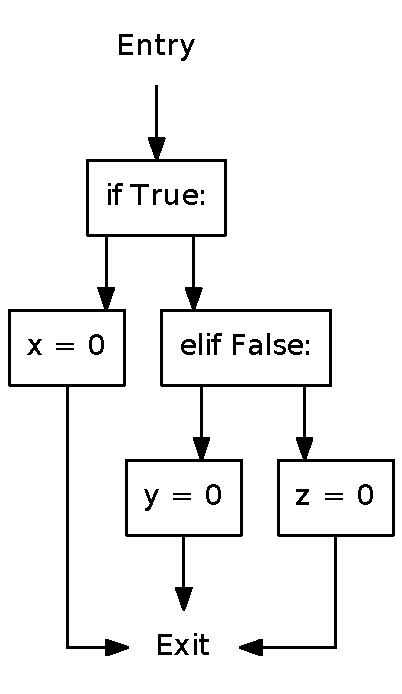
\includegraphics[scale=.5]{./figures/if_else_elif.pdf}
    \caption{Possible flows}
    \label{CFG_if_flow}
  \end{subfigure}

  \caption{An AST and the expected CFG}
  \label{CFG_if_else}  
\end{figure}

\subsection{From AST to CFG}
Implementing the CFG requires considering all the cases mentioned in \cref{python:control_structures}.
\Cref{CFG_if_else} shows an one of the cases with the intermediate AST step included (\cref{CFG_if_ast}).
Here the AST is visualised as a tree, where the first node is an \texttt{If} node\footnote{An AST for a complete program starts with a \texttt{Module} node, but this is not shown here in order to simplify the tree}
This node contains a test node, a body, represented as a list of nodes, and an orelse body, also represented as a list of nodes.
In this example the conditions are \texttt{NameConstant} nodes and all statements are \texttt{Assign} nodes.
The orelse body of the outer \texttt{If} node contains another \texttt{If} node which contains the \texttt{elif} which has the else in its orelse body.

The CFG of the program is generated by traversing the AST and creating a CFG node at each node.
These nodes are then connected so the resulting CFG reflects the flow of the program.
The implementation of the \texttt{If} visitor will be described in the following.

\subsection{Visitor implementation}\label{cfg:visitor}
\Cref{visit_if_code} shows the implementation of visiting an \texttt{If} AST node.
First, another visitor, the \texttt{LabelVisitor} is used to find labels of statements in the CFG.
In \cref{if_test_label} it is used to generate the label of the condition in the \texttt{if}.
Afterwards a CFG node is created for the condition and appended to the list of CFG nodes.
In \cref{if_body_handling} the body of the \texttt{if} is handled by the \texttt{stmt\_star\_handler} method.
This method visits all nodes in the body and connects them properly.
\Cref{if_orelse_handling} now handles \texttt{elif} and \texttt{else} cases.
Again \texttt{stmt\_star\_handler} handles the connection of the bodies.

Through the implementation a number of 'last nodes' are being kept track of.
This is for instance seen in \cref{if_last_statements} where the 'last nodes' of the orelse node are added to the 'last nodes' of the body.
A 'last statement' is in this context any statement that needs to be connected to the subsequent statement of the \texttt{if}.
Among these are \texttt{raise} statements, \texttt{return} statements and the last statements of the body, \texttt{elif} bodies and the \texttt{else} body.
These are sent to the calling function by returning a \texttt{ControlFlowNode} in \cref{if_return}.
This calling function is \texttt{stmt\_star\_handler} which, as stated above, connects all the nodes properly.

\begin{lstlisting}[style=python, caption={Visiting an If AST node.}, label={visit_if_code}, escapeinside={(*@}{@*)}, breaklines=true]
def visit_If(self, node):
    label_visitor = LabelVisitor() (*@\label{if_test_label}@*)
    label_visitor.visit(node.test)

    test = self.append_node(Node(label_visitor.result, node, line_number = node.lineno))
    self.add_if_label(test)

    body_connect_stmts = self.stmt_star_handler(node.body) (*@ \label{if_body_handling} @*)
    test.connect(body_connect_stmts.first_statement)
        
    if node.orelse: (*@ \label{if_orelse_handling} @*)
        orelse_last_nodes = self.handle_or_else(node.orelse, test)
        body_connect_stmts.last_statements.extend(orelse_last_nodes) (*@ \label{if_last_statements} @*)
    else:
        body_connect_stmts.last_statements.append(test)

    last_statements = self.remove_breaks(body_connect_stmts.last_statements)

    return ControlFlowNode(test, last_statements, break_statements=body_connect_stmts.break_statements) (*@ \label{if_return} @*)
\end{lstlisting}

\section{Framework adaptor}\label{framework_adaptor}
Our goal of our tool is to target web application frameworks.
As there exist different frameworks and these are organised in different manners, we need to accommodate for these variations.
The framework adaptor is purposed to accommodate for different web application frameworks.
The \texttt{FrameworkAdaptor} class is an abstract class with an abstract method \texttt{run}.
It contains a list of CFGs where the adaptor is expected to put the result of the adaptation.
The implementation of \texttt{run} should include processing for all framework specific details that are needed in order to get a correct model of the application.
This adaptor can be implemented for an arbitrary framework like Django or, in our case, Flask.

\paragraph{The Flask Adaptor}
In Flask all web pages are defined in a function with a decorator.
This function is never explicitly called in the source code, so a single traversal by the CFG visitor of the file will not include all these methods in the resulting list of CFGs.
The adaptor \texttt{FlaskAdaptor} was implemented for this purpose.
The result of the CFG visitor contains all functions found during the traversal.
The Flask adaptor goes through these and finds all functions that are defined with the \texttt{@app.route()} decorator, and adds it to the list of CFGs.
This results in a list of CFGs that cover all the code needed for analysing the application.

\paragraph{Implementing a custom adaptor}
The adaptor component is in place for making it possible to adapt the analysis to any framework.
This section will describe how such an implementation should be devised.

In \cref{appendix:flask_adaptor} the implementation of the Flask adaptor is shown.
This implementation will be used as a basis for this description.
The adaptor inherits from the class \texttt{FrameworkAdaptor} which contains an instance variable for a CFG list and the abstract function \texttt{run}.
The \texttt{run} function is the entry point to an adaptor.

In the Flask implementation the CFG list, which is initially populated with the result of the CFG visitor, is iterated over and the \texttt{find\_flask\_route\_functions} function is called on each. \footnote{In our case there is always one CFG in this list, but other implementations might have more than one.}
The idea of the \texttt{find\_flask\_route\_functions} was described in the previous paragraph.
A similar consideration has to be made for the framework in question and then implemented in a similar fashion.

After implementing a custom adaptor, \pyt{} will be able to analyse any application using this framework.
  


\section{Flexible analysis}\label{impl:flexible}
As mentined in \cref{impl:overview} the fixed point analysis is implemented so that the analysis can be changed.
For our purposes the \emph{reaching definitions} analysis is sufficient -- it provides the answers we need to locate the security vulnerabilities in web applications.

However, one could imagine improving \pyt{} by utilizing other analyses that could help identify the vulnerabilities.
In such a case \pyt{} has been implemented so it can be easiliy expanded with another analysis.
The liveness analysis presented in \citet[p.~19]{schwartzbach} has been implemented in order to exemplify the process of implementing new analyses.
This process will be explained in the following.

\subsection{Implementing liveness}
The complete implementation is presented in \cref{appendix:liveness}.
The implementation corresponds to the definition presented in \citet[p.~20]{schwartzbach}.
The \texttt{LivenessAnalysis} class inherits from \texttt{AnalysisBase} which contains logic for annotating the CFG with extra information.
In the case of the liveness analysis we need information about the \texttt{vars(E)} of each node.
The deduction of these are defined as a visitor \texttt{VarsVisitor} \todo{maske ref til visitor som bliver omtalt på et tidspunkt} which visits an AST node and finds the variables as defined in \citet{schwartzbach}.

\texttt{LivenessAnalysis} contains the constraints of the liveness analysis defined in \texttt{fixpointmethod}, which is shown in \cref{liveness_impl_fixpointmethod}.
This method is used by the fixed point analysis to apply the constraints on each node.
This method uses a helper \texttt{JOIN} which corresponds to the JOIN function in \citet{schwartzbach}, and the variables found by \texttt{VarsVisitor}.

\begin{lstlisting}[style=python, caption={Implementation of liveness analysis - \texttt{fixpointmethod}}, label={liveness_impl_fixpoint}, escapeinside={(*@}{@*)}, firstnumber=24]
    def fixpointmethod(self, cfg_node):
        """Setting the constraints of the given cfg node
        obeying the liveness analysis rules."""
    
        # if for Condition and call case: Join(v) u vars(E).
        if cfg_node.ast_type == Compare.__name__ or
           cfg_node.ast_type == Call.__name__:
            JOIN = self.join(cfg_node)
            # set union
            JOIN.update(self.annotated_cfg_nodes[cfg_node])  
            cfg_node.new_constraint = JOIN

        # if for Assignment case: Join(v) \ {id} u vars(E).
        elif isinstance(cfg_node, AssignmentNode): 
            JOIN = self.join(cfg_node)
            # set difference
            JOIN.discard(cfg_node.ast_node.targets[0].id)
            # set union
            JOIN.update(self.annotated_cfg_nodes[cfg_node])  
            cfg_node.new_constraint = JOIN

        # if for entry and exit cases: {}.
        elif cfg_node.ast_type == "ENTRY" or
             cfg_node.ast_type == "EXIT":
            pass
        # else for other cases.
        else:
        cfg_node.new_constraint = self.join(cfg_node)
\end{lstlisting}

With this implementation the \pyt{} fixed point algorithm implementation can perform liveness analysis on an arbitrary piece of python source code.
The \pyt{} vulnerability checker could likewise be expanded with any analysis that could aid the detection of security vulnerabilites.

\section{Vulnerabilities}
This module uses the result of the fixed-point analysis to detect vulnerabilities in the application.

\paragraph{Trigger word definition}
A definition file is provided that contains sources, sinks and sanitisers which are used to find vulnerabilities in the source code.
A simple text file with two keywords  is used for this purpose.
The keywords ``sources:'' and ``sinks:'' are used to indicate the content of the section.
Each source or sink is written on a separate line.
A sink can have a number of sanitisers attached written with as a comma separated list after an arrow (``\texttt{->}'').
Sinks, sources and sanitisers are called trigger words, and the definition file is called a trigger word file, and an example can be seen in \cref{trigger_word_file}.
\begin{lstlisting}[style=default, caption={How the trigger word file should be defined.}, label={trigger_word_file}]
  sources:
  source_1
  source_2

  sinks:
  sink_1
  sink_2 -> sanitiser_1
  sink_3 -> sanitiser_1, sanitiser_2, sanitiser_3
\end{lstlisting}

\paragraph{Finding and logging vulnerabilities}
After parsing the file all potential vulnerabilities are found and saved in a log.
The concept of finding vulnerabilities was described in \cref{theory_finding_vulns}.
Vulnerabilities are found by first identifying all nodes which contain a trigger word.
All sources are then checked if their constraint contain a source, and i that is the case, if a sanitiser is in between the two.
These cases are then logged to the vulnerability log.
A \texttt{Vulnerability} is an object which consists of a source and a sink CFG node, and which words triggered the detection of these.
A source and a sink have attached a line number to them, this line number tells where they are located in the source code.
This information is used to make it as easy as possible for the developer to find and determine whether the vulnerability found is harmful.
An example of a vulnerability log can be found in \cref{vulnerability_log_example}.
The output shown is after running \pyt{} on \cref{xss}.
The vulnerability is reported by showing details of both source and sink, with the relevant trigger word and the line number in the source code.
This should enable the developer to either fix the vulnerability or assess it as being safe.

\begin{lstlisting}[style=default, caption={An example of how the vulnerability log looks after it found one vulnerability.}, label={vulnerability_log_example}]
1 vulnerability found:
Vulnerability 0:
User input at line 8, trigger word "get": 
    param = request.args.get('param', 'not set')
reaches line 11, trigger word "replace": 
    resp = make_response(html.replace('{{ param }}', param))
\end{lstlisting}

\section{Sources, sinks and  and sanitisers in Flask}
In order to find dangerous flows in a program we need to know what expressions introduce user input and what expressions may not receive input.
We also need to be able to detect when the program actually makes such input harmless.

An expression which introduces user input in some way is called a \emph{source}, while a dangerous destination for such input is called a \emph{sink}.
A function that can neutralise input so it is not dangerous to send to a sink is called a \emph{sanitiser}.

\begin{lstlisting}[style=python, caption={A simple vulnerable program}, label=simple_sink_source]
x = input()
print('this is dangerous!')
eval(x)
\end{lstlisting}

The program in \cref{simple_sink_source} is vulnerable to a user executing arbitrary code.
\texttt{input()} is a source and \texttt{eval()} is a sink.
The result of \texttt{input()} is being handed over to \texttt{eval()} without any sanitisation.
Imagine this program being served on a server which also contains confidential information.
An attacker would possibly be able to retrieve this confidential information from the server.

\subsection{Flask}
Flask is a web framework, so it uses some different means of user input than the \texttt{input()} method.
This section will cover a selection of these in order to have a basis for performing an analysis of a Flask application.

\paragraph{Sources}
In \cref{flask:intro} the \texttt{request} object was introduced.
This object is used to access the input provided by the user through interaction with the page.

\subparagraph{Query parameters}
Query parameters submitted to the URL can be accessed with the \texttt{request.args.get(key, default)} method.
This method takes the key to retrieve a value from and a default value as parameters.
If this methods returns a value that is different from the default, it is potentially dangerous.

\subparagraph{Form content}
Input submitted through form fields can be accessed with the \texttt{request.form[key]} attribute.
This attribute is a dictionary that maps a form field to its value.
Values retrieved from this dictionary are potentially dangerous.

\paragraph{Sinks}
User input can arrive at a wealth of methods which can be regarded as a sink.
We explored three vulnerabilities in \cref{security_vulnerabilities} which we would like to be able to detect.
The following is the sinks that can possibly enable the chosen vulnerabilities.
These are obviously only a small selection of all possible sinks.

\subparagraph{Homemade templates}
When utilising the template engine of Flask many security concerns are ruled out.
An eager developer that is too impatient to read the documentation for \emph{Jinja2} may resort to a solution that works, but is subpar regarding security.
One example of this could be to use \texttt{string.replace(old, new)} instead of the template engine.
The developer creates his own template format, and replaces placeholders with user input.
It works, but if the input does not get sanitised, the user can inject javascript into the page, see \cref{vulnerabilities:xss}.

The input passed to \texttt{string.replace()} can be sanitised using the \texttt{Markup} class provided by Flask.
\texttt{Markup} is used to represent HTML markup and marks them as being safe.
It contains an \texttt{escape} function that escapes HTML tags and thereby sanitises the input.
Manipulating a markup object with string interpolation also escapes all values.
An example of escaping user input can be seen on \cref{escape} where the \texttt{Markup.escape} method is used to sanitise the input before inserting it with the \texttt{string.replace()} method.

\begin{lstlisting}[style=python, caption={An example of escaping user input}, label={escape}]
  html = open('templates/example1.html').read()
  unsafe = request.args.get(param)

  sanitised = Markup.escape(unsafe)
  
  resp = make_response(html.replace('{{ param }}', sanitised))
\end{lstlisting}


\subparagraph{Database access}
db.engine.execute filter format trick

\todo{ref til vulnerabilities:injection}
\subparagraph{Filesystem access}
Files can be sent to the client with the \texttt{send\_file(filename)} method.
This method takes a file from the filesystem and sends it to the user.
If the filename parameter is set by user input, the user can possibly traverse the filesystem of the server, see \cref{vulnerabilities:traversal}.
This can be sanitised by disallowing the use of '..' in the variable passed to the filename parameter.

\section{\pyt}
This section contains a description of how to use \pyt{}.
\pyt{} is a command line tool which requires one argument, the path of the file that should be analysed, and several optional arguments.
These are described below.

\subsection{Positional Arguments}
\pyt{} requires one positional argument, \texttt{filepath}, which is the path of the file which should be analysed.
If the file is a part of a project the folder in which the file is in is used as root.
To specify another root one can use the optional argument \texttt{--project-root} explained below in \cref{pyt:optional}.

\subsection{Optional Arguments}\label{pyt:optional}
This section contains a brief description of the optional arguments of \pyt{}.
\todo{Tjek at den er liste passer med den endelige udgave af pyt.}

\paragraph{Project Root}
The project root argument is used for specifying the root of the project when the filepath given is not in the root folder of the project.

\paragraph{Draw CFG}
This argument is useful to visualise a CFG.
It outputs a PDF file that contains a graph like the one on \cref{theory:general_code_example_cfg}.

\paragraph{Output Filename}
This argument can be used to specify the output name of the file that is generated when using the \texttt{--draw-cfg} or the \texttt{--create-database} argument.

\paragraph{Print}
This outputs the CFG to the standard output in simple representation.
This prints all labels of each node in the CFG.

\paragraph{Verbose Print}
The same as the print argument but more verbose.
This means that all information a node contains is send to the output.

\paragraph{Trigger Word File}
This argument is used for specifying a trigger word file which is a file as defined in \cref{impl:vulnerabilities}.
This is optional as per default the Flask trigger word file that comes with \pyt{}.

\paragraph{Log Level}
This argument is used for setting the log level of the logger that is used.
The log level can be changed to the following levels, highest level first: CRITICAL, ERROR, WARNING, INFO, DEBUG or NOTSET.
Setting the log level will result in the log containing messages from the chosen level and the levels above.
The default log level is \texttt{WARNING} and the logger writes the output of the logging to a text file ``logger.log''.

\paragraph{Adaptor}
This argument is used for specifying a framework adaptor.
Per default \pyt{} uses the Flask adaptor which comes with it, see \cref{framework_adaptor}.

\paragraph{Create Database}
\todo{write when implemented :b}

\paragraph{Help}
This options shows a short overview of the available arguments and their meaning.
On \cref{tool_overview} the output of running \pyt{} with this argument is depicted.

\begin{figure}
  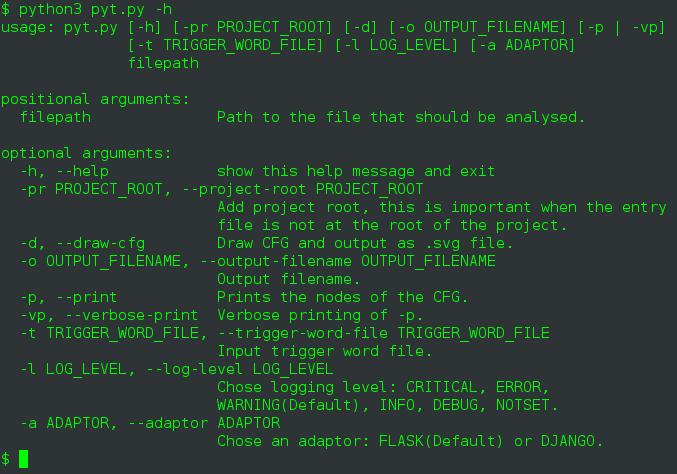
\includegraphics[width=\textwidth]{./figures/pyt_overview.png}
  \caption{An overview of \pyt{} and its arguments.}
  \label{tool_overview}
\end{figure}


\subsection{Command line argument summary}
\Cref{pyt:arguments_overview} shows a quick overview of the arguments of \pyt{} and the corresponding flags to use when running the tool.

\newcommand{\pytarg}[2]{
  \texttt{#1} & #2.
}
\begin{figure}
  \begin{tabular}{l | l}
    \textbf{Argument} & \textbf{Description} \\
    \hline
    \pytarg{filepath}{Specify path of file to analyse} \\
    \pytarg{-pr, --project-root}{Specify project root} \\
    \pytarg{-d, --draw-cfg}{Draw CFG and output as a PDF file} \\
    \pytarg{-o, --output-filename}{Name of the file that is output} \\
    \pytarg{-p, --print}{Prints a CFG with simple information about the nodes} \\
    \pytarg{-vp, --verbose-print}{Same as print but with all information about the nodes} \\
    \pytarg{-t, --trigger-word-file}{Specify a trigger word file} \\
    \pytarg{-l, --log-level}{Set a log level} \\
    \pytarg{-a, --adaptor}{Chose an adaptor} \\
    \pytarg{-db, --create-database}{Create a sql file of the CFG} \\
    
\end{tabular}
  \centering
  \caption{\pyt{}s arguments.}
  \label{pyt:arguments_overview}
\end{figure}

\section{Limitations}
\subsection{Dynamic Features}
The following dynamic features are not supported meaning that the right flow of the source code is not captured and therefore is not taken into account in the analysis.
\pyt{} does not support the built in functions \texttt{eval} and \texttt{exec}.
These functions take a string as input which are executed as Python code.
This means that the content of this string cannot be evaluated statically, and \pyt{} cannot anticipate what will happen.

\pyt{} does also not support monkey patching.
Monkey patching is used to replace functions in order to manipulate modules or classes.
This is powerful but also difficult to capture.

Not supporting the above dynamic features means that taint can be introduced without \pyt{} noticing.
One way to fix this is to overtaint by just tainting all nodes containing \texttt{eval} and \texttt{exec} for instance.

\subsection{Decorators}
Decorators are used to transform a function into another function.
Flask uses this to register functions that should be accessible as a webpage.
In practice a decorator is implemented as a class that contains a transformation function that returns the transformed function.
When a function definition is decorated, the transformed function will be used instead.
An example was provided in \cref{python:decorators}.

The current implementation do not perform this decoration process.
A decorated definition is not transformed, and the decorator is stored.
This means that some details may be lost.
Some transformations may introduce taint, which will not be caught by \pyt{}.

A correct implementation of decorators will be very similar to that of a function call, but there will be some considerations on how to capture the transformed function correctly.

\subsection{Libraries}
The import handling does its best to find the implementation of functions called throughout the program, but it can only find the implementation of functions where the source code is available.
This may be limiting the analysis, but having to traverse all library code will be a major task.
Fixing this requires considerations of when it is worth doing, and when it is just increasing running time, without adding value.

\subsection{Language Constructs}
This section contains a list of language constructs that were not implemented due to time constraints and were not deemed important as most of them were not faced in the projects we ran as input.
Language constructs not implemented:
\begin{itemize}
\item \textbf{Async} - used for asynchronous programming.\cite{python_async}
\item \textbf{Decorators} - used for function transformations, explained in \cref{python:decorators}.
\item \textbf{Try} - used for catching exceptions.\cite{python_exception}
\item \textbf{Delete} - a statement to delete a name.\cite{python_delete}
\item \textbf{Assert} - a statement that can be used to insert debugging assertions into a program.\cite{python_assert}
\item \textbf{Global} - a statement that declares a name global so that one can access global names from other scopes.\cite{python_global}
\item \textbf{Yield} - used in generator functions to ``return'' one item at a time.\cite{python_yield}
\item \textbf{Starred} - used for unpacking (only partially implemented).\cite{python_unpacking}
\end{itemize}


\section{Testing}
During the development of the application we have had great success working test oriented.
In particular when developing the conversion from abstract syntax tree to control flow graph, testing has been invaluable.
The abstract nature of the syntax tree together with the many possibilities of python yield a huge number of cases for each construct, and the edges have to be just right in every one of them.

When developing all these fragments of the complete grammar, we need to be sure that our previous work still works as intended.
To help us be sure that all our assumptions and implementations hold we have utilised unit testing a great deal.
The following will mention some of the issues where testing has helped the process.

\paragraph{Cases}
An example of a construct which has many different cases is the \texttt{if} control structure, which has variants with \texttt{elif} and \texttt{else} statements.
The \texttt{if} abstract syntax node contains an \emph{orelse} reference which can either be another \texttt{if}, representing an \text{elif} clause, or a list of statements, representing the body of an \texttt{else} clause.
In addition an \texttt{if} can have many different expressions in its \emph{test} clause.
These expressions are often logic expressions but can also be nameconstants, function calls, lambdas and even a list.
To illustrate the three d\texttt{if}ferent cases three abstract directed graphs have been made.
\begin{itemize}
\item The graph for a single \texttt{if} statement can be seen on the left on \cref{test:ast:if_and_else}.
\item The graph for an \texttt{if} and an \texttt{elif} statement can be seen on the right on \cref{test:ast:if_and_else}.
\item The graph for an \texttt{if}, \texttt{elif} and else statement can be seen on \cref{test:ast:if_elif_else}
\end{itemize}
\textbf{Note:} On \cref{test:ast:if_and_else} and \cref{test:ast:if_elif_else}, \textit{expr} is an expression and \textit{stmt*} is a list of statements.


\begin{figure}
    \begin{subfigure}[b]{0.45\textwidth}
        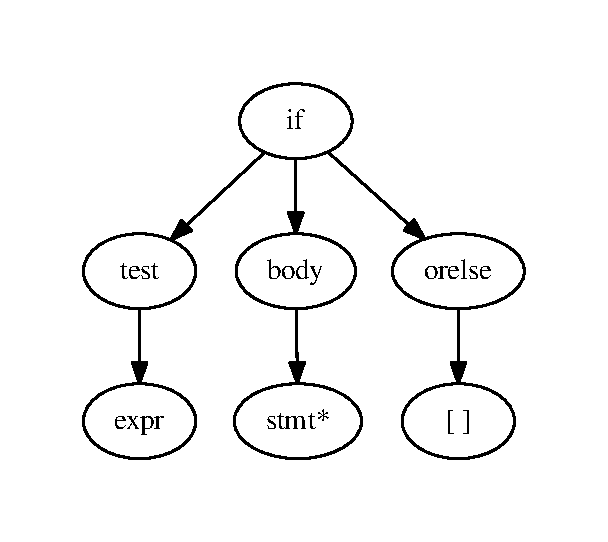
\includegraphics[width=\textwidth]{./figures/dot_files/if_ast.pdf}
    \end{subfigure}
    ~ %add desired spacing between images, e. g. ~, \quad, \qquad, \hfill etc. 
    %(or a blank line to force the subfigure onto a new line)
    \begin{subfigure}[b]{0.45\textwidth}
        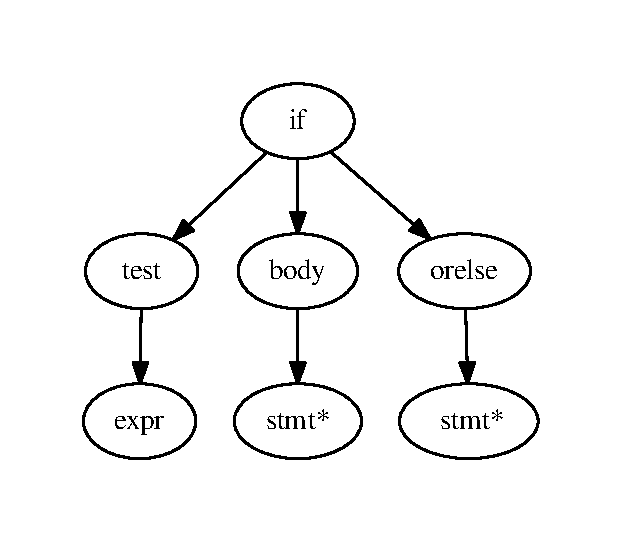
\includegraphics[width=\textwidth]{./figures/dot_files/if_else.pdf}
    \end{subfigure}
    \caption{Abstract graph showing the nodes in the abstract syntax tree for a single \texttt{if} statement on the left and an \texttt{if} and \texttt{else} statement on the right.}
    \label{test:ast:if_and_else}
\end{figure}

\begin{figure}
  \centering
  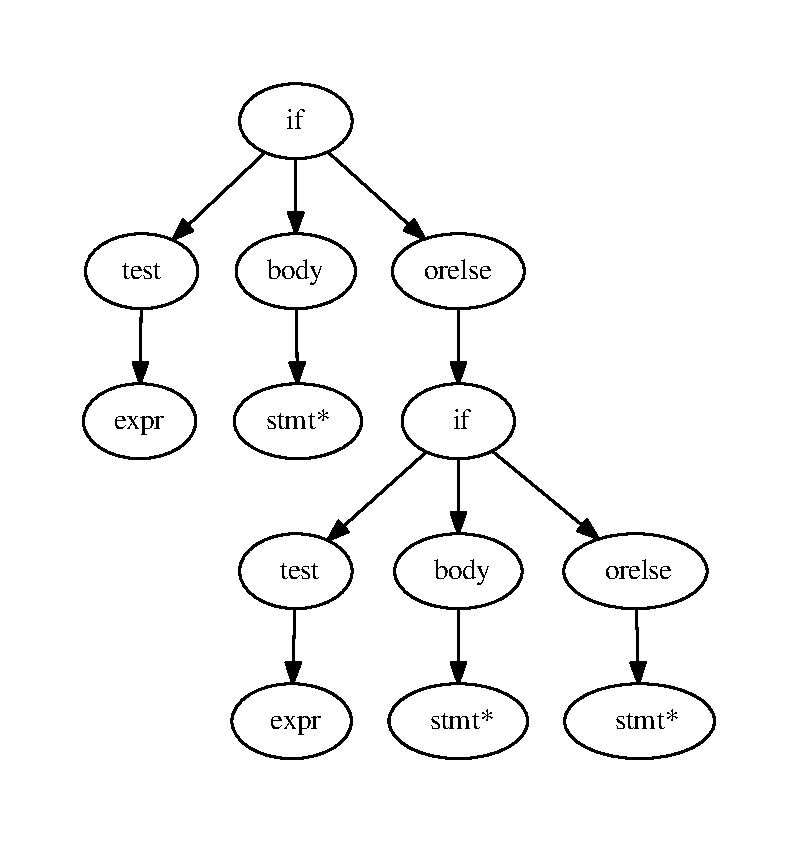
\includegraphics[scale=.7]{./figures/dot_files/if_elif_else.pdf}
  \caption{Abstract graph showing the nodes in the abstract syntax tree for an \texttt{if},\texttt{elif} and \texttt{else} statement.}
  \label{test:ast:if_elif_else}
\end{figure}

When the basic cases of the \texttt{if} is implemented we also need to know that \texttt{if} statements inside the body of an \texttt{if} statement works properly.
When that works we need to consider how to handle \texttt{break}, \texttt{yield} and \texttt{return} statements inside the \texttt{if}.

Testing has greatly helped when exploring and developing these cases, because they explicitly run each case every time the test is run.
This assures that a change fixing one case did not break another case.

\paragraph{Complex features}
The development of python is still ongoing which results in periodic changes to both the grammar and the semantics of the language.
Continuously adding features from both the object oriented and the functional paradigm results in more possibilities but also a more complex internal structure.
This is evident when attempting to generate control flow graphs from the abstract syntax.

One example is that you can assign a list to a tuple, and python will \emph{unpack} and assign the items of the list to the corresponding items of the tuple.
This is possible using the \texttt{*}-operator.
An example is show on \cref{tuple:unpacking}, where x is assigned the value 4 and the tuple y is overwritten with the list [5, 6].
\begin{lstlisting}[style=python, caption={Tuple unpacking}, label=tuple:unpacking]
  x = 1
  y = (2,3)
  x,*y = [4,5,6]
\end{lstlisting}

Generating the control flow graph for expressions like these have given a lot of insight into python, but it has also been a challenge to represent them properly in the control flow graph.
Also here testing has provided useful for keeping track of the parts involved.
The example consists of assignments, a tuple, the star operator and a list in order to show off one concept.
All the concepts both need to work individually and together, and tests have helped ensuring this.

\paragraph{Dynamic types}
Python is a dynamic language which can be very unforgiving to debug.
A wrong type returned from a function produces an error in a function somewhere completely different.
The stack trace is not always helpful at telling where the actual problem is located.

When developing with tests a catalogue of small tests are naturally developed.
When introducing an error that breaks more than just the construct at hand, test have helped pinpointing the real cause of the error.
This has sometimes lead to insight that either helped us understand why our implementation was wrong, or why what we expected was not the real outcome.


\chapter{Discussion}
\section{Evaluation}
This section will contain an evaluation of \pyt{}.
First the vulnerabilities described in \cref{security_vulnerabilities} will be run and serve as proof that the tool catches these vulnerabilities.
Thereafter \pyt{} will be run on real projects and the performance of the tool will be evaluated.

\subsection{Detecting manufactured vulnerabilities}
In \cref{security_vulnerabilities} we presented four implementation mistakes that would leave a web application vulnerable.
In this section the resuling tool, \pyt{}, will be run on the presented examples to see if they are being detected as hoped.

\paragraph{SQL injection}
The first example was the SQL injection which can be found in \cref{appendix:sqli}.
Here we expect to find the two vulnerabilities presented in \cref{vulnerabilities:sqli}, the naive execution of the query parameter and the unescaped filter.

As seen on \cref{sqli:console} we get a report with two vulnerabilities.
The first one detected is the filtering vulnerability.
\pyt{} tells us that the trigger word 'get' was found in line 33, which then reached line 36 where the trigger word 'filter' marked it as a sink.

The second one is the naive implementation of the database query.
Here the vulnerability is reported to begin at line 26 where the trigger word 'get' pointed out a sink.
This sink then reaches line 27 where the trigger word 'execute' indicates a sink.

Both vulnerabilities were thus able to be found by \pyt{}.

\begin{figure}
  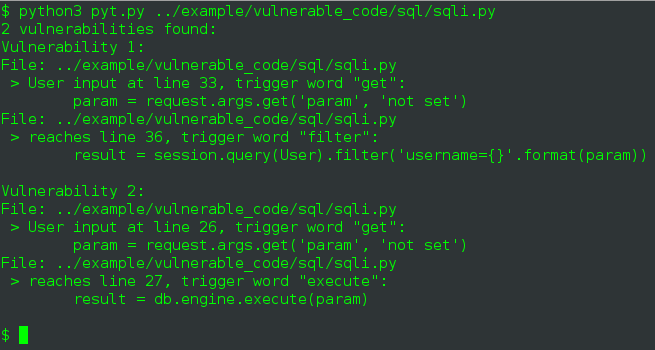
\includegraphics[width=\textwidth]{./figures/sqli_console.png}
  \caption{Running \pyt{} on the SQL injection example}
  \label{sqli:console}
\end{figure}

\paragraph{Command injection}
The next example was the command injection which can be found in \cref{appendix:command_injection}.
Here we expect to find the one vulnerability presented in \cref{vulnerabilities:ci} where the content of the form field reaches the subprocess call.

The execution of \pyt{} on the example can be seen on \cref{ci:console}.
\pyt{} reports one vulnerability being present in the application.
A source is found on line 15 with the trigger word 'form', which reaches a sink in line 18 marked because of the trigger word 'subprocess.call'.
In this case the source was assigned to a new variable in line 16 to make up the complete command to be run.
This is shown by \pyt{} as to provide information to the developer of how the tainted value did flow through the code.
  
\begin{figure}
  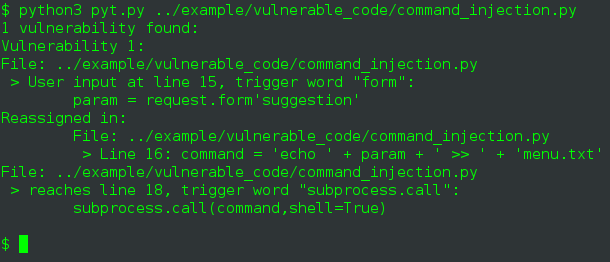
\includegraphics[width=\textwidth]{./figures/command_injection_console.png}
  \caption{Running \pyt{} on the command injection example}
  \label{ci:console}
\end{figure}

\paragraph{Cross site scripting}
The next vulnerability presented was the cross site scripting attack described in \cref{vulnerabilities:xss}.
The code can be found in \cref{appendix:xss}.

The execution of \pyt{} on the example can be seen on \cref{xss:console}.
Here a source is found in line 6 with the trigger word 'get', which reaches the sink in line 9 with the trigger word 'replace'.
Notice that the vulnerability reports a reassignment in line 10 which is irrelevant to the vulnerability because it happens after the sink.
Also notice that the reported line looks different than the source line because of the CFG representation of a return node.
This can potentially be confusing for the user of \pyt{}.

\begin{figure}
  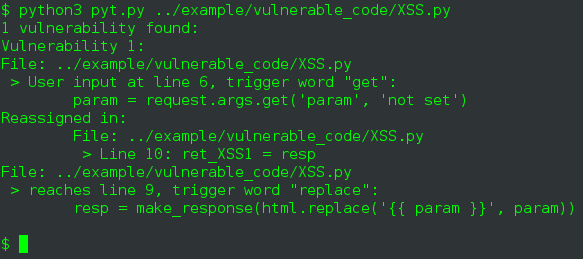
\includegraphics[width=\textwidth]{./figures/xss_console.png}
  \caption{Running \pyt{} on the XSS example}
  \label{xss:console}
\end{figure}

\subparagraph{Sanitised cross site scripting example}
As mentioned in \cref{theory_finding_vulns} some vulnerabilities can be sanitised by special functions, making the dangerous code harmless.
Running \pyt{} on the sanitised version presented in \cref{sanitised_xss} results in the output presented in \cref{xss_sanitised:console}

Here the vulnerability is found as in the above, but it concludes the vulnerability report by adding that it is potentially sanitised by the 'escape' function.

\begin{figure}
  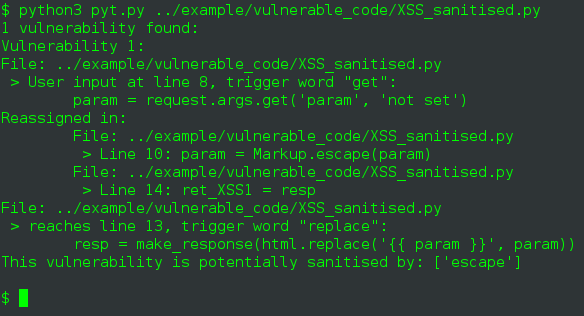
\includegraphics[width=\textwidth]{./figures/xss_sanitised_console.png}
  \caption{Running \pyt{} on the sanitised XSS example}
  \label{xss_sanitised:console}
\end{figure}

\paragraph{Path traversal}
The final vulnerability presented was the path traversal.
The code can be found in \cref{appendix:path_traversal}.
In this example we expect to find the vulnerability presented in \cref{vulnerabilities:traversal}.

The execution of \pyt{} on the example is shown in \cref{path_traversal:console}.
Here the report shows one vulnerability, starting with a sink found in line 8 with the trigger word 'get'.
This source then reaches the sink in line 11 which is detected by the trigger word 'send\_file'.

\begin{figure}
  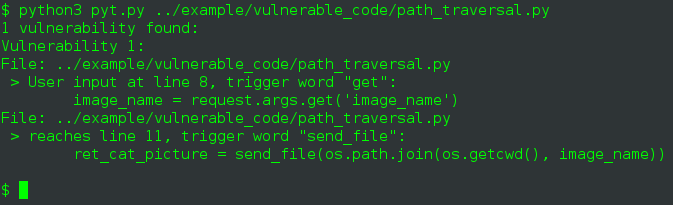
\includegraphics[width=\textwidth]{./figures/path_traversal_console.png}
  \caption{Running \pyt{} on the Path traversal example}
  \label{path_traversal:console}
\end{figure}

\subsection{Detecting vulnerabilities in real projects}
\todo{DETECT}

\subsection{Summary}
\todo{maybe a summary of the results?}

\section{Reflections}
This chapter will reflect on \pyt{} and the experiences we have had during the development of the tool.

\subsection{Are Frameworks like Flask Good for Web Security?}
In the beginning of the project period we had an idea of making a tool that could find security flaws in web applications.
We were well aware that vulnerabilities would not be in an abundance.
Even when looking at lists of well known vulnerabilities, these were hard to apply to Flask applications.
Flask takes care of a lot without the user even having to think about it.

We therefore had to resort to the vulnerabilities we presented in \cref{security_vulnerabilities}.
These vulnerabilities are still dangerous, but could be unlikely to be found in the wild. (Maybe with the exception of the command injection vulnerability. This may actually be valid for some cases.)

Our experience with the Flask framework is therefore an indication that frameworks like Flask definitely help security of web applications.

\section{Future Works}
This section contains a number of subjects which can be improved upon and worked on in the future.

\subsection{Better Trigger Word Definitions}
Finding sources and sinks was a feature where the literature was sparse.
Plenty of papers use the terms, but no one described a clever way to find them.
We therefore devised our own system.

The implemented system uses a text file with the trigger words written in a very simple syntax.
The labels of CFG nodes are compared with the trigger words, and if they contain one, they are marked as being either a source, a sink or a sanitiser.
Using this simple implementation we ran into problems like finding the trigger word in variable names.
The quick solution was to add a '(' to the trigger word, which fixed that single problem.

In further development the whole trigger word system should be reconsidered.
The definition should be more sophisticated, and the comparison should be more intelligent than just comparing in the label.

\subsection{More Vulnerability Definitions}
One of the reasons that our evaluation found no vulnerabilities in real applications (see \cref{evaluation}), is the small number of vulnerabilities \pyt{} looks for.
The used trigger word definition file only finds those particular vulnerabilities that was found in the beginning of the project.
In order to make \pyt{} really useful, this trigger word definition should be expanded, not only with new vulnerabilities, but also with variants of the vulnerabilities already being searched for.
The two SQL injection attacks presented in \cref{vulnerabilities:sqli} is one example of a vulnerabilities where variants of the same vulnerability exists.
It is imaginable that many vulnerabilities exists in a number of variants that all need to be defined by trigger words.

\subsection{More Efficient Fixed-point Algorithm}
In this project efficiency has not been a priority, and for the most part is has not been a problem.
In the evaluation performed on real projects, described in \cref{evaluation:real}, this suddenly became a hurdle.
It turns out that big projects produce CFGs that are so large that \pyt{} simply does not terminate in a realistic amount of time.
It would therefore be a natural next step to attempt to improve this inefficiency.
As mentioned in \cref{fixed_point_algorithm} this project has not spent time examining alternative implementations of the fixed-point algorithm.
One suggestion would therefore be to attempt to implement the improved version of the algorithm, in order to get a faster analysis.

\subsection{Expanding \pyt{} with Other Analyses}
As discussed in \cref{impl:flexible}, \pyt{} has been implemented in a flexible way, so that any analysis can be implemented.
This means that it is possible to expand the analysis with supporting analyses.
The implemented example, liveness analysis, could be used to determine if a found vulnerability is in a piece of dead code.
If this is the case, the developer might not be interested in this particular vulnerability.
The danger of not displaying vulnerabilities in dead code is of course that this code may become live at any time, and then the vulnerability is suddenly dangerous.
There could therefore be a optional command line flag that filters out dead code, based on the liveness analysis.

Other analyses could also prove helpful in the detection of vulnerabilities.

\subsection{Support More Frameworks}
This project has only looked into the Flask web framework.
In order to make \pyt{} even more useful, more frameworks should be supported.
As mentioned in \cref{preliminaries:web_frameworks}, Django is a very popular framework.
Implementing support for Django could greatly increase the number of applications that \pyt{} is able to analyse.

Implementing another framework requires a new adaptor.
The process of writing a new framework adaptor was described in \cref{framework_adaptor}.


\chapter{Conclusion}
\chapter{Conclusion}\label{ch:conclusion}
In case you have questions, comments, suggestions or have found a bug, please do not hesitate to contact me. You can find my contact details below.
  \begin{center}
    Jesper Kjær Nielsen\\
    \href{mailto: jkn@es.aau.dk}{jkn@es.aau.dk}\\
    \href{http://kom.aau.dk/~jkn}{http://kom.aau.dk/\textasciitilde jkn}\\
    Fredrik Bajers Vej 7\\
    9220 Aalborg Ø
  \end{center}


\appendix
\chapter{Vulnerability implementations}

\section{SQL injection}\label{appendix:sqli}
\begin{lstlisting}[numbers=left, frame=single, escapeinside={(*@}{@*)}]
from flask import Flask, request
from flask_sqlalchemy import SQLAlchemy
import sys

app = Flask(__name__)

# SQL Alchemy setup
app.config['DATABASE_URI'] = 'sqlite:////tmp/test.db'
db = SQLAlchemy(app)

class User(db.Model):
    id = db.Column(db.Integer, primary_key=True)
    username = db.Column(db.String(80), unique=True)
    email = db.Column(db.String(120), unique=True)

    def __init__(self, username, email):
        self.username = username
        self.email = email

    def __repr__(self):
        return '<User %r>' % self.username    
    
@app.route('/')
def index():
    param = request.args.get('param', 'not set')
    result = db.engine.execute(param) (*@ \label{sql1} @*)
    print(User.query.all(), file=sys.stderr) 
    return 'Look console'

@app.route('/value_injection')
def value():
    param = request.args.get('param', 'not set')
    result = db.engine.execute(
        'select * from User where username = "'
        + param + '";') (*@ \label{sql2} @*)
    for row in result:
        print(row, file=sys.stderr)
    return 'Look console'


if __name__ == '__main__':
    app.run(debug=True)
\end{lstlisting}


\section{XSS}\label{appendix:xss}
\begin{lstlisting}[numbers=left, frame=single, escapeinside={(*@}{@*)}]
from flask import Flask, render_template,
                  request, make_response
import random
import string
app = Flask(__name__)

@app.route('/')
def home():
    return "Hello, World!"  # return a string

html = open('templates/example1.html').read()

@app.route('/example1', methods =['GET'])
def example1():
    param = request.args.get('param', 'not set')
    resp = make_response(html.replace('{{ param }}', param))
    resp.set_cookie(
        'session_id',
        ''.join(random.choice(string.ascii_uppercase)
        for x in range(16)))
    return resp

@app.route('/example2')
def example2():
    return render_template('example2_form.html')

html1 = open('templates/example2_response.html').read()

@app.route('/example2action',methods = ['POST'])
def example2_action():
    data = request.form['my_text'] (*@ \label{xss:request} @*)
    resp = make\_response(html1.replace('{{ data }}', data )) (*@ \label{xss:replace}@*)
    resp.set_cookie(
        'session_id',
        ''.join(random.choice(string.ascii_uppercase)
        for x in range(16)))
    return resp

if __name__ == '__main__':
    app.run(debug= True)
\end{lstlisting}


\section{Path Traversal}\label{appendix:path_traversal}
\begin{lstlisting}[numbers=left, frame=single, escapeinside={(*@}{@*)}]
import os
from flask import Flask, redirect, request, send_file

app = Flask(__name__)

@app.route('/')
def cat_picture():
    image_name = request.args.get('image_name')
    if not image_name:
        return 404
    return send_file(os.path.join(os.getcwd(), image_name)) (*@ \label{traversal:path} @*)


if __name__ == '__main__':
    app.run(debug=True)
\end{lstlisting}


\chapter{Implementation of the liveness analysis}\label{appendix:liveness}

\begin{lstlisting}[style=python, caption={Implementation of liveness analysis}, label={liveness_impl}, escapeinside={(*@}{@*)}]
"""Module implements liveness analysis."""
from cfg import AssignmentNode
from copy import deepcopy
from ast import NodeVisitor, Compare, Call

from analysis_base import AnalysisBase

class LivenessAnalysis(AnalysisBase):
    """Implement liveness analysis rules."""

    def __init__(self, cfg):
        """Initialize using parent with the given cfg."""
        super(LivenessAnalysis, self).__init__(cfg, VarsVisitor)
    
    def join(self, cfg_node):
        """Join outgoing old constraints
        and return them as a set."""
        JOIN = set()
        for outgoing in cfg_node.outgoing:
            if outgoing.old_constraint:
                JOIN |= outgoing.old_constraint
        return JOIN
    
       def fixpointmethod(self, cfg_node):
        """Setting the constraints of the given cfg node
        obeying the liveness analysis rules."""
    
        # if for Condition and call case: Join(v) u vars(E).
        if cfg_node.ast_type == Compare.__name__ or
           cfg_node.ast_type == Call.__name__:
            JOIN = self.join(cfg_node)
            # set union
            JOIN.update(self.annotated_cfg_nodes[cfg_node])  
            cfg_node.new_constraint = JOIN

        # if for Assignment case: Join(v) \ {id} u vars(E).
        elif isinstance(cfg_node, AssignmentNode): 
            JOIN = self.join(cfg_node)
            # set difference
            JOIN.discard(cfg_node.ast_node.targets[0].id)
            # set union
            JOIN.update(self.annotated_cfg_nodes[cfg_node])  
            cfg_node.new_constraint = JOIN

        # if for entry and exit cases: {}.
        elif cfg_node.ast_type == "ENTRY" or
             cfg_node.ast_type == "EXIT":
            pass
        # else for other cases.
        else:
        cfg_node.new_constraint = self.join(cfg_node)
        

class VarsVisitor(NodeVisitor):
    """Class that finds all variables needed
    for the liveness analysis."""

    def __init__(self):
        """Initialise list of results."""
        self.result = list()

    def visit_Name(self, node):
        self.result.append(node.id)

    #  Condition and call rule
    def visit_Call(self, node):
        for arg in node.args:
            self.visit(arg)
        for keyword in node.keywords:
            self.visit(keyword)
            
    def visit_keyword(self, node):
        self.visit(node.value)

    def visit_Compare(self, node):
        self.generic_visit(node)

    #  Assignment rule                
    def visit_Assign(self, node): 
        self.visit(node.value)          
\end{lstlisting}

\chapter{The Abstract Syntax of Python}\label{appendix:abstract_syntax}
The following shows the complete abstract syntax of the python programming language.
It is taken directly from \citet{ast_python}.

\begin{lstlisting}[style=default, caption={The abstract syntax of Python}, label={python_abstract_syntax}, breaklines=true]
-- ASDL's six builtin types are identifier, int, string, bytes, object, singleton

module Python
{
    mod = Module(stmt* body)
        | Interactive(stmt* body)
        | Expression(expr body)

        -- not really an actual node but useful in Jython's typesystem.
        | Suite(stmt* body)

    stmt = FunctionDef(identifier name, arguments args,
                       stmt* body, expr* decorator_list, expr? returns)
          | AsyncFunctionDef(identifier name, arguments args,
                             stmt* body, expr* decorator_list, expr? returns)

          | ClassDef(identifier name,
             expr* bases,
             keyword* keywords,
             stmt* body,
             expr* decorator_list)
          | Return(expr? value)

          | Delete(expr* targets)
          | Assign(expr* targets, expr value)
          | AugAssign(expr target, operator op, expr value)

          -- use 'orelse' because else is a keyword in target languages
          | For(expr target, expr iter, stmt* body, stmt* orelse)
          | AsyncFor(expr target, expr iter, stmt* body, stmt* orelse)
          | While(expr test, stmt* body, stmt* orelse)
          | If(expr test, stmt* body, stmt* orelse)
          | With(withitem* items, stmt* body)
          | AsyncWith(withitem* items, stmt* body)

          | Raise(expr? exc, expr? cause)
          | Try(stmt* body, excepthandler* handlers, stmt* orelse, stmt* finalbody)
          | Assert(expr test, expr? msg)

          | Import(alias* names)
          | ImportFrom(identifier? module, alias* names, int? level)

          | Global(identifier* names)
          | Nonlocal(identifier* names)
          | Expr(expr value)
          | Pass | Break | Continue

          -- XXX Jython will be different
          -- col_offset is the byte offset in the utf8 string the parser uses
          attributes (int lineno, int col_offset)

          -- BoolOp() can use left & right?
    expr = BoolOp(boolop op, expr* values)
         | BinOp(expr left, operator op, expr right)
         | UnaryOp(unaryop op, expr operand)
         | Lambda(arguments args, expr body)
         | IfExp(expr test, expr body, expr orelse)
         | Dict(expr* keys, expr* values)
         | Set(expr* elts)
         | ListComp(expr elt, comprehension* generators)
         | SetComp(expr elt, comprehension* generators)
         | DictComp(expr key, expr value, comprehension* generators)
         | GeneratorExp(expr elt, comprehension* generators)
         -- the grammar constrains where yield expressions can occur
         | Await(expr value)
         | Yield(expr? value)
         | YieldFrom(expr value)
         -- need sequences for compare to distinguish between
         -- x < 4 < 3 and (x < 4) < 3
         | Compare(expr left, cmpop* ops, expr* comparators)
         | Call(expr func, expr* args, keyword* keywords)
         | Num(object n) -- a number as a PyObject.
         | Str(string s) -- need to specify raw, unicode, etc?
         | Bytes(bytes s)
         | NameConstant(singleton value)
         | Ellipsis

         -- the following expression can appear in assignment context
         | Attribute(expr value, identifier attr, expr_context ctx)
         | Subscript(expr value, slice slice, expr_context ctx)
         | Starred(expr value, expr_context ctx)
         | Name(identifier id, expr_context ctx)
         | List(expr* elts, expr_context ctx)
         | Tuple(expr* elts, expr_context ctx)

          -- col_offset is the byte offset in the utf8 string the parser uses
          attributes (int lineno, int col_offset)

    expr_context = Load | Store | Del | AugLoad | AugStore | Param

    slice = Slice(expr? lower, expr? upper, expr? step)
          | ExtSlice(slice* dims)
          | Index(expr value)

    boolop = And | Or

    operator = Add | Sub | Mult | MatMult | Div | Mod | Pow | LShift
                 | RShift | BitOr | BitXor | BitAnd | FloorDiv

    unaryop = Invert | Not | UAdd | USub

    cmpop = Eq | NotEq | Lt | LtE | Gt | GtE | Is | IsNot | In | NotIn

    comprehension = (expr target, expr iter, expr* ifs)

    excepthandler = ExceptHandler(expr? type, identifier? name, stmt* body)
                    attributes (int lineno, int col_offset)

    arguments = (arg* args, arg? vararg, arg* kwonlyargs, expr* kw_defaults,
                 arg? kwarg, expr* defaults)

    arg = (identifier arg, expr? annotation)
           attributes (int lineno, int col_offset)

    -- keyword arguments supplied to call (NULL identifier for **kwargs)
    keyword = (identifier? arg, expr value)

    -- import name with optional 'as' alias.
    alias = (identifier name, identifier? asname)

    withitem = (expr context_expr, expr? optional_vars)
}
\end{lstlisting}


\printbibliography
\end{document}
